%Unrelated: "timed games"


%*** General probabilistic notation ***

\newcommand{\expv}{\mathbf{E}} % EXP. VALUE
\newcommand{\discProbDist}{f} % Discrete prob distribution
\newcommand{\sampleSpace}{S} % Generic sample space
\newcommand{\sigmaAlg}{\mathcal{F}} % Generic sigma-algebra
\newcommand{\probm}{\mathbb{P}} % Generic probability measure, also prob. measure operator
\newcommand{\rvar}{X} % Generic random variable
%\newcommand{\dist}{\mathit{Dist}}

%*** MDP notation ***

\newcommand{\actions}{A} % The set of actions.
\newcommand{\colouring}{c} % the colouring function
\newcommand{\probTranFunc}{\Delta} % Transition function of an MDP
\newcommand{\edges}{E} % Set of edges in an MDP.
\newcommand{\colours}{C} % The set of colours in an MDP.
\newcommand{\mdp}{\mathcal{M}} % A generic MDP. 
\newcommand{\vinit}{v_0} % An initial vertex in an MDP.
\newcommand{\cylProb}{p} % Function assigning probabilities to cylinder sets in 
%the measure construction.
\newcommand{\emptyPlay}{\epsilon} %empty play
\newcommand{\objective}{\Omega} % Qualitative objective
\newcommand{\genColour}{\textsc{c}} % Generic colour
\newcommand{\quantObj}{f} % Generic quantitative objective
\newcommand{\indicator}[1]{\mathbf{1}_{#1}} % In.d RV
\newcommand{\eps}{\varepsilon} % Numerical epsilon
\newcommand{\maxc}{W} % Maximal abs. value of a colour

\newcommand{\winPos}{W_{>0}}
\newcommand{\winAS}{W_{=1}}
\newcommand{\cylinder}{\mathit{Cyl}}

\newcommand{\PrePos}{\text{Pre}_{>0}}
\newcommand{\PreAS}{\text{Pre}_{=1}}

\newcommand{\PreOPPos}{\mathcal{P}_{>0}}
\newcommand{\OPAS}{\mathcal{P}_{=1}}

\newcommand{\safeOP}{\mathit{Safe_{=1}}}
\newcommand{\closed}{\mathit{Cl}}

\newcommand{\reachOP}{\mathcal{V}}
\newcommand{\discOP}{\mathcal{D}}
\newcommand{\valsigma}{\vec{x}^{\sigma}}

\newcommand{\lp}{\mathcal{L}}
\newcommand{\lpdisc}{\lp_{\mathit{disc}}}
\newcommand{\lpmp}{\lp_{\mathit{mp}}}
\newcommand{\lpsol}[1]{\bar{#1}}
\newcommand{\lpmpdual}{\lpmp^{\mathit{dual}}}

\newcommand{\actevent}[3]{\actions^{#1}_{#2,#3}} % Returns #1-th action on the run 

\newcommand{\MeanPayoffSup}{\MeanPayoff^{+}}
\newcommand{\MeanPayoffInf}{\MeanPayoff^{-}}

\newcommand{\mcprob}{M}
\newcommand{\invdist}{\vec{z}}

\newcommand{\hittime}{T}



This chapter studies two-player games whose arena is defined by a pushdown system\footnote{We use here the term pushdown system rather than pushdown automaton to stress the fact that we are not considering these devices as language acceptors but rather focus on the transitions systems they define.}. The vertices of the arena are the configurations of the pushdown system (i.e., pairs composed of a control state and a word representing the content of the stack) and the edges of the arena are defined by the pushdown system's transitions. For simplicity, both the ownership of a configuration and the objective will only depend on the control state of the configuration. Hence the partition of all the configurations between the two players will simply be given by a partition the control states. We will mainly consider the parity objective. Via a standard reduction\AC{Insert a reference to a previous chapter.}, parity pushdown game can be used to solve any pushdown game with an $\omega$-regular objectives (which in our setting is simply an $\omega$-regular set of infinite words over  the alphabet of control states). 

The main conceptual novelty of this chapter is that the arena is no longer finite. However as these games are described by a finite amount of information: the pushdown system, the ownership partition and the $\omega$-regular objective, they are amenable to algorithmic treatment. The first natural problem in this line is to decide the winner of the game from a given configuration. We will also consider the computation of \emph{finite representations} for the winning regions and the winning strategies. 


\section{Basic Definitions}
%\begin{itemize}
%%\item Graphs (if needed)
%%\item Pushdown automata
%%\item Pushdown graphs (coming with examples). Probably with labels on the edges. Notion of configuration.
%%\item Pushdown games (coming again with examples; in particular one showing that the attractor may not converge in finite time, \emph{i.e.} transfinite induction is needed
%\item Stating the main questions: deciding whether a configuration is winning; computing a finite presentation of the winning region; computing a finite presentation of a winning strategy (stress that even if positional the strategy may be problematic to present).
%\item Notion of finite presentation of infinite objects. The notion for winning regions is quite clear : regular sets and the notion for strategies is less immediate: pushdown automaton, regular sets for each action, optimal strategies in reachability game does not work.
%\end{itemize}


A \emph{pushdown system} is a tuple $\PDS = (Q,Q_{\mEve}, Q_{\mAdam}, \Gamma,\Delta,C)$\AC{Do we add $\pdscol{}$ and $\bot$ to the tuple of a pushdown system ? I have no opinion.} 
where:
\begin{itemize} 
	\item $Q$ is a finite set of control states with $Q = Q_{\mEve} \uplus Q_{\mAdam}$ which is partionned between the two players \Eve and \Adam. Moreover with each state $q$ is associated a colour $\pdscol{q} \acchanged{\in C}$;	\item $\Gamma$ is the stack alphabet. There is a special bottom-of-stack symbol, denoted $\bot$, which does not belong to $\Gamma$; we let $\Gamma_\bot$ denote the alphabet $\Gamma \cup \set{\bot}$;
	\item $\Delta:Q\times \Gamma_\bot\rightarrow 2^{Q\times\{\pop,\push{\gamma}\mid \gamma\in\Gamma\}}$ is the transition relation. We additionally require that for all states $p,q\in Q$, $(q,\pop)\notin\Delta(p,\bot)$, i.e., the bottom of stack symbol is never popped.
\end{itemize}

We call a pair $(p,s)\in Q \times \bot\Gamma^*$ a \emph{configuration} of $\PDS$: $p$ is the control state of the configuration while $s$ is its stack content. We let $\sh((p,s))=|s|-1$ denote the \emph{stack height} of the  configuration $(p,s)$. \acchanged{Intuitively, if $(q,\push{\gamma'})$ belongs to $\Delta(p,\gamma)$, the pushdown system
in any configuration of the form $(p,s\gamma)$ can go to state $q$ after pushing the symbol $\gamma$ on top of the stack, leading to the configuration $(q,s\gamma\gamma')$. Similarly, if $(q,\pop)$ belongs to $\Delta(p,\gamma)$, the pushdown system
in any configuration of the form $(p,s\gamma)$ can go to the configuration $(q,s)$ after \emph{poping} the top symbol from the stack.}
% \end{definition}

%A configuration of $\PDS$ is a pair $(q,s)\in Q\times \bot \Gamma^*$.

A pushdown system induces an arena $\arena = (G,\VE,\VA)$ called a \emph{pushdown arena} where
\begin{itemize}
	\item the set of vertices is the set $V = Q \times \bot\Gamma^* $ of configurations of $\PDS$ with $\VE = Q_{\mEve} \times \bot\Gamma^*$ 
	and $\VA = Q_{\mAdam} \times \bot\Gamma^* $;
	\item the set $E$ of edges induced by $\Delta$ is
\begin{equation*}
\begin{split}
	E  = & \{((p,s\gamma),\pdscol{p},(q,s)) \mid (q,\pop)\in\Delta(p,\gamma)\}\quad \cup \\ 
	&  \{((p,s\gamma),\pdscol{p},(q,s\gamma\gamma')) \mid (q,\push{\gamma'})\in\Delta(p,\gamma)\}.
\end{split}	
\end{equation*}
\end{itemize}

% TODO : Dans la conclusion, il faut parler d'autres formes de conditions de gain comme l'explosion de pile.

\acchanged{
\begin{remark}
In this chapter, we deviate slightly from the general setting used in the book as we colour vertices and not edges. 
Because we only consider qualitative objectives, it is more convenient to consider the equivalent setting where we label vertices by colours rather than edges which is the usual convention in pushdown games.  
In the definition of a pushdown arena, the colour of an edge is uniquely determined by the colour of the control state of the source vertex. Therefore,  we also view in this chapter plays as sequences of vertices rather than sequences of edges.
\end{remark}
}


Finally, a \emph{pushdown game} is a game played on a pushdown arena. In this chapter we only consider qualitative objectives of the form $\Omega\subseteq C^\omega$ \acchanged{where $C$ is the set of colours. As in our definition, 
colours are associated to control states, the objective we consider only depend on the sequence of control states of the configurations visited along a play. By a slight abuse of notation, for a play $\pi \in V^*$, we let $\pi=(p_1,s_1)(p_2,s_2)\cdots \in \Omega$ denotes the fact that the sequences of colours $(\pdscol{p_i})_{i\geq 1}$ belongs to $\Omega$.} %\OS{Dans la conclusion discuter d'autres conditions mais l\`a c'est plus confort}



\begin{example}\label{11-ex:pushdown-game-1}
Consider the pushdown system $\PDS = (Q,Q_{\mEve}, Q_{\mAdam}, \Gamma,\Delta)$ where:
\begin{itemize}
	\item $Q_{\mEve}=\{q,r\}$ and $Q_{\mAdam}=\{p\}$; $\pdscol{p} = 1$, $\pdscol{q} = 2$ and $\pdscol{r} = 0$.
	\item $\Gamma=\{\gamma\}$ is a singleton.
	\item $\Delta(p,\bot) = \{(p,\push{\gamma})\}$, $\Delta(p,\gamma) = \{(p,\push{\gamma}),(q,\pop)\}$, $\Delta(q,\bot) = \{(r,\push{\gamma})\}$, $\Delta(q,\gamma) = \{(q,\pop)\}$ and $\Delta(r,\gamma) = \{(q,\pop)\}$.
\end{itemize}

\Cref{11-fig:example-pushdown-game-1} depicts the part of the pushdown arena $\arena$ induced by $\PDS$ when restricted to the vertices reachable from $(p,\bot)$.

Consider the reachability game $(\arena, \Reach(\{0\}))$. Then, every vertex of the form $(q,\bot v)$ is winning for \Eve and every vertex of the form $(p,\bot v)$ is winning for \Adam as \Adam can always choose to push a $\gamma$-symbol while remaining in state $p$ hence always avoiding the state $r$ (which is the only state with colour $0$). If instead we consider, the B{\"u}chi game $\Buchi(\{0,2\})$, then \Eve is winning form all vertices. The strategy for \Adam consisting in always pushing a $\gamma$-symbol while remaining in state $p$ results in a play that infinitely often sees the colour $2$.

\begin{figure}[htb]
\begin{center}
\begin{tikzpicture}[>=stealth',thick,scale=1,transform shape]
\tikzstyle{Adam}=[draw,inner sep=4]
\tikzstyle{Eve}=[draw,rounded rectangle,inner sep=4]
\tikzstyle{Nature}=[draw,diamond,scale = .65,font=\Large]
\tikzstyle{AdamH}=[]
\tikzstyle{EveH}=[circle]
\tikzset{every loop/.style={min distance=10mm,looseness=10}}
\tikzstyle{loopleft}=[in=150,out=210]
\tikzstyle{loopright}=[in=-30,out=30]
\node[Adam] (A1) at (1,0) {$(p,\bot)$};
\node[Adam] (A2) at (3.2,0) {$(p,\bot\gamma)$};
\node[Adam] (A3) at (5.5,0) {$(p,\bot\gamma\gamma)$};
\node[Adam] (A4) at (7.7,0) {$(p,\bot\gamma\gamma\gamma)$};
\node[AdamH] (A5) at (9.6,0) {};
%%
\node[Eve] (E0) at (-1,-1.5) {$(r,\bot\gamma)$};
\node[Eve] (E1) at (1,-1.5) {$(q,\bot)$};
\node[Eve] (E2) at (3.2,-1.5) {$(q,\bot\gamma)$};
\node[Eve] (E3) at (5.5,-1.5) {$(q,\bot\gamma\gamma)$};
\node[Eve] (E4) at (7.7,-1.5) {$(q,\bot\gamma\gamma\gamma)$};
\node[EveH] (E5) at (9.6,-1.5) {};



%\path[->] (A1) edge node[above] {$1$}   (A2);
%\path[->] (A2) edge node[above] {$1$} (A3);
%\path[->] (A2) edge node[above] {$1$}(A3);
%\path[->] (A3) edge node[above] {$1$}(A4);
%\path[->,dotted] (A4) edge node[above] {$1$}(A5);
%
%\path[->] (A2) edge node[above] {$1$} (E1);
%\path[->] (A3) edge node[above] {$1$} (E2);
%\path[->] (A4) edge node[above] {$1$} (E3);
%\path[->,dotted] (A5) edge node[above] {$1$}(E4);
%
%\path[->] (E0) edge[bend right] node[below] {$0$} (E1);
%\path[->] (E1) edge node[above] {$2$} (E0);
%\path[->] (E2) edge node[above] {$2$} (E1);
%\path[->] (E3) edge node[above] {$2$} (E2);
%\path[->] (E4) edge node[above] {$2$} (E3);
%\path[->,dotted] (E5) edge node[above] {$2$}(E4);

\path[->] (A1) edge    (A2);
\path[->] (A2) edge  (A3);
\path[->] (A2) edge (A3);
\path[->] (A3) edge (A4);
\path[->,dotted] (A4) edge (A5);

\path[->] (A2) edge (E1);
\path[->] (A3) edge (E2);
\path[->] (A4) edge (E3);
\path[->,dotted] (A5) edge (E4);

\path[->] (E0) edge[bend right]  (E1);
\path[->] (E1) edge (E0);
\path[->] (E2) edge (E1);
\path[->] (E3) edge (E2);
\path[->] (E4) edge (E3);
\path[->,dotted] (E5) edge (E4);




%\path[->,bend right] (N2) edge (N1);
\end{tikzpicture}
\end{center}
\caption{Pushdown arena from \Cref{11-ex:pushdown-game-1}}\label{11-fig:example-pushdown-game-1}
\end{figure}

\end{example}


As a pushdown arena is in general infinite, the \emph{winning region} for \Eve, i.e., the set of winning vertices for \Eve may not admit a finite presentation. Similarly, for objectives for which finite-memory strategies exists, the question of whether such a strategy can be finitely presented (and computed) is raised. Hence, we will in general distinguish the following three algorithmic problems.

\begin{svgraybox}
For pushdown games, ``solving the game'' means solving the following decision problem:
\vskip1em
\decisionproblem{A pushdown game $\game$ and an initial vertex $v_0$}{Does Eve win $\game$ from $v_0$?}
\end{svgraybox}


\begin{svgraybox}
For pushdown games, ``computing the winning region'' means solving the following problem:
\vskip1em
\begin{tabular}{rl}
	\textbf{INPUT:} & A pushdown game $\game$ \\
	\textbf{OUTPUT:} & A finite presentation of the set $v$ of vertices from which  Eve wins $\game$
\end{tabular}
\end{svgraybox}

In \Cref{11-thm:regularity-wr}, we will show that the winning region can be described by a finite-state automaton  for a large class of qualitative winning conditions.

\begin{svgraybox}
For pushdown games, ``computing a winning strategy'' means solving the following problem:
\vskip1em
\begin{tabular}{rp{9.5cm}}
	\textbf{INPUT:} & A pushdown game $\game$ \\
	\textbf{OUTPUT:} & A finite presentation of a strategy for \Eve that is winning from any vertex in the winning region for Eve in $\game$
\end{tabular}
\end{svgraybox}

%\OSlong{compl\'eter}

We will show, for parity pushdown games, that the winning strategy can be described using either a finite-state automaton (see \Cref{11-section:regular-strat}) or a pushdown automaton (see \Cref{11-section:pushdown-strat}).


\section{Profiles and Regularity of the Winning Region}

In this section, we consider a large class of objectives called \emph{prefix independent}. For these objectives, a pushdown game can be meaningfully decomposed by considering the part of the game between the moment a symbol is pushed onto the stack and stopping as soon as it is popped.  As a consequence, we will see that for prefix independent
objectives, the winning region can be described  using finite state automata.




%\subsection{Profiles}
\acchanged{To this extent, we introduce \emph{reduced games} which start with a stack containing only one symbol $\gamma$ and stop as soon as this symbol is popped from the stack. If the symbol is never popped, the objective is unchanged and otherwise the winner of the game is determined by the state reached when popping the symbol.}

Let $\game=(\arena,\Omega)$ be a pushdown game played on an arena $\arena = (G,\VE,\VA)$ generated by a pushdown system $\PDS = (Q,Q_{\mEve}, Q_{\mAdam}, \Gamma,\Delta)$. For any subset $R\subseteq Q$ of control states of $\PDS$, we define a new objective $\Omega(R)$ such that a play $\play$ belongs to $\Omega(R)$ if one of the following happens:
%\begin{itemize}
%\item  In $\play$ no configuration with an empty stack, {i.e.} of the form $(q,\bot)$, is visited, and $\play\in\Omega$.
%\item In $\play$ a configuration with an empty stack is visited and the control state in the first such configuration belongs to $R$.
%\end{itemize}
\acchanged{
\begin{itemize}
\item the play $\play$ belongs to $\Omega$ and does not contain
any configuration with an empty stack ( {i.e.}, of the form $(q,\bot)$ for some state $q \in Q$),
\item the play $\play$ contains a configuration with the empty stack and the first such configuration has a state in R.
\end{itemize}}


More formally, letting $V=V_\mEve\cup V_\mAdam$, $V_R = R \times \bot \Gamma^*$ and $V_\bot = Q \times \{\bot\}$ 
$$ \Omega(R) = (\Omega \setminus V^*V_\bot V^\omega)\cup (V \setminus V_\bot)^* V_R V^\omega$$
Finally, we let $\game(R)$ denote the game $(\arena,\Omega(R))$.

\acchanged{Remark that contrarily to the rest of the objectives considered in this chapter, $\Omega(R)$ does depend on the sequences of vertices visited by the play and not only on their colour. It would have been possible by a slight modification of the arena to only express the objective on their colours. However, our choice simplifies the presentation of the reduced games.}

For any state $q\in Q$ and any stack letter $\gamma\in\Gamma$, we denote by $\mathcal{R}(q,\gamma)$ the set of subsets $R\subseteq Q$ for which \Eve wins in $\game(R)$ from $(q,\bot\gamma)$:
$$\mathcal{R}(q,\gamma)=\{
R\subseteq Q\mid (q,\bot\gamma) \text{ is winning for \Eve in } \game(R)
\}$$ and we refer to $\mathcal{R}(q,\gamma)$ as the \emph{$(q,\gamma)$-profile} of $\game$.

An objective $\Omega\subseteq C^\omega$ is \emph{prefix independent} if the following holds: for every $u\in C^\omega$ and for every \acchanged{$v\in C^*$},  $u\in \Omega$ if and only if $vu\in \Omega$. The Büchi, co-Büchi and parity objectives are examples of prefix independent objectives and the reachability objective is not.


\begin{remark} 
\label{11-rem:stay-staying-alive}
For a prefix independent objective, a play respecting a winning strategy for $\Eve$ that starts in \Eve's winning region always stay in this region. Obviously this is no longer true if the objective is not prefix independent. For instance in a reachability game, a play following a winning strategy for $\Eve$ can leave the winning region of \Eve once the target has been reached. 	
\end{remark}


This simple property allows to use profiles to give an inductive characterization of the winning region for \Eve when the objectif is prefix independent.

\begin{proposition}\label{11-prop:returning} Assume that $\Omega\subseteq C^\omega$ is prefix independent. 
Let $s\in \Gamma^*$, $q\in Q$ and $\gamma\in\Gamma$. Then \Eve has a winning strategy in $\game$ from $(q,\bot s\gamma)$ if and only if there exists some $R\in\mathcal{R}(q,\gamma)$ such that $(r,\bot s)$ is winning for \Eve in $\game$ for every $r\in R$.
\end{proposition}

\begin{proof}
Assume \Eve has a winning strategy $\sigma$ from $(q,\bot s\gamma)$ in $\game$. Consider the set $\Pi_\sigma$ of all plays in $\game$ that starts from $(q,\bot s\gamma)$ and where \Eve respects $\sigma$. Define $R$ to be the (possibly empty) set that consists of all $r\in Q$ such that there is a play in $\Pi_\sigma$ of the form $v_0\cdots v_k (r,\bot s) v_{k+1}\cdots$ where each $v_i$ for $0\leq i\leq k$ is of the form $(p_i,\bot s t_i)$ for some non-empty $t_i$. In other words, $R$ consists of all states that can be reached on popping $\gamma$ for the first time in a play where \Eve respects $\sigma$. As seen in \cref{11-rem:stay-staying-alive}, \Eve is winning from $(r,\bot s)$ for all $r \in R$. It remains to show that $R\in\mathcal{R}(q,\gamma)$.

To this end, define a (partial) function $\xi$ as $\xi((p,\bot s t))=(p,\bot t)$ for every $p\in Q$ and set $\xi^{-1}((p,\bot t))=(p,\bot s t)$. Then $\xi^{-1}$ is extended as a morphism over $V^*$.  Now a winning strategy for \Eve in $\game(R)$ is defined as follows:
\begin{itemize}
\item if some empty stack configuration has already been visited play any valid move, 
\item otherwise go to $\xi(\sigma(\xi^{-1}(\pi))$, where $\pi$ is the current play.
\end{itemize}
By definition of $\Pi_\sigma$ and $R$, it easily follows that the previous strategy is winning for \Eve in $\game(R)$, and therefore $R\in\mathcal{R}(p,\gamma)$. 
%Finally, for every $r\in R$ there is, by definition of $\Pi_\sigma$ a finite play $\pi_r$ that starts from $(q,\bot s\gamma)$, where \Eve respects $\sigma$ and that ends in $(r,\bot s)$. A winning strategy for \Eve in $\game$ from $(r,\bot s)$ is given by $\sigma'(\pi)=\sigma(\pi'_r\pi)$, where $\pi'_r$ denotes the partial play obtained from $\pi_r$ by removing its last vertex $(r,\bot s)$.

Conversely, let us assume that there is some $R\in\mathcal{R}(q,\gamma)$ such that $(r,\bot s)$ is winning for \Eve in $\game$ for every $r\in R$. For every $r\in R$, let us denote by $\sigma_r$ a winning strategy for \Eve from $(r,\bot s)$ in $\game$. Let $\sigma_R$ be a winning strategy for \Eve in $\game(R)$ from $(q,\bot\gamma)$. Let us define $\xi$ and $\xi^{-1}$ as in the direct implication and extend them as (partial) morphism over $V^*$. Define the following strategy $\sigma$ for \Eve in $\game$ for plays starting from $(q,\bot s\gamma)$. For any such play $\pi$, 
\begin{itemize}
\item if $\pi$ does not contain a configuration of the form $(p,\bot s)$ then we take $\sigma(\pi)=\xi^{-1}(\sigma_R(\xi(\pi)))$;
\item otherwise let $\pi = \pi'\cdot(r,\bot s)\cdot \pi''$ where $\pi'$ does not contain any configuration of the form $(p,\bot s)$. If $r$ does not belong to $R$, $\sigma$ is undefined. Note that this situation will never be encountered in a play respecting $\sigma$ as $\sigma_R$ ensures that $r \in R$. If $r \in R$, one finally sets $\sigma(\pi)=\sigma_r((r,\bot s)\pi'')$.
\end{itemize} 
The strategy $\sigma$ is a winning strategy for \Eve in $\game$ from $(q,\bot s\gamma)$. To see this, consider a play $\pi$ starting from $(p,\bot s \gamma)$ and respecting $\sigma$.

 If the play $\pi$ does not contain configurations of the form $(r,\bot s)$ for some $r \in Q$, then the play $\xi(\pi)$ starting in $(p,\bot \gamma)$ respects $\sigma_R$ and is won by $\Eve$.
As $\xi(\pi)$ does not contain configurations with an empty stack, it must be the case that $\xi(\pi) \in \Omega$. As $\Omega$ only depends on the colours of the states, it is also the case that $\pi \in \Omega$ and hence, $\pi$ is winning for $\Eve$. 

If the play $\pi$ can be decomposed as $\pi' (r,\bot s) \pi''$ where $\pi'$ does not contain any configuration with the stack $\bot s$, the play $\xi(\pi' (r,\bot s))$ respects $\sigma_R$ in $\game(R)$. As $\sigma_R$ is winning, it follows that $r \in R$. By definition of $\sigma$, $(r,\bot s)\pi''$ respects $\sigma_r$ which being winning for \Eve implies that $(r,\bot s) \pi'' \in \Omega$. As $\Omega$ is prefix independent, it follows that $\pi \in \Omega$.
\end{proof}

%Consider a quantitative objective $\Omega\subseteq C^\omega$. 

\Cref{11-prop:returning} implies that the winning region of any pushdown game equipped with a prefix independent objectives can be described by regular languages.

\begin{theorem}\label{11-thm:regularity-wr}
Let $\game=(\arena,\Omega)$ be a pushdown game played on an arena $\arena = (G,\VE,\VA)$ generated by a pushdown system $\PDS = (Q,Q_{\mEve}, Q_{\mAdam}, \Gamma,\Delta)$, and such that $\Omega\subseteq C^\omega$ is prefix independent. Then for any state $q\in Q$, the set \[
L_q=\{u\in \Gamma^*\mid (q,\bot s)\in W_\mEve \}
\] is a regular language over the alphabet $\Gamma$.
\end{theorem}

\begin{proof}
Fix a control state $q \in Q$, we consider a deterministic finite state automaton defined as follows. Its set of control states consists of the subsets of $Q$ and the initial state is $S_{in}=\{p\mid (p,\bot)\in W_\mEve\}$. From the state $S$ upon reading the letter $\gamma$ the automaton goes to the state $\{p\mid S\in\mathcal{R}(p,\gamma)\}$. Finally a state $S$ is final if and only if $q\in S$. It is then an immediate consequence of \Cref{11-prop:returning} that this automaton accepts the language $L_q$.
\end{proof}


\begin{remark}\label{11-rk:automata-winning-region}
By a slight abuse, we can think of the $|Q|$ automata in \Cref{11-thm:regularity-wr}	as a single automaton that is design to first read the stack content and finally reads the control state $q$ (in this latter step, from state $S$ it either go to a final state if $q\in S$ or to a rejecting one otherwise).
\end{remark}


\begin{remark}
Note that the characterisation in \Cref{11-thm:regularity-wr} is \emph{a priori} not effective. Indeed, to construct automata for the languages $L_q$ one needs to be able to compute all the $(q,\gamma)$-profiles $\mathcal{R}(q,\gamma)$ of $\game$ and compute
the winner from configurations of the form $(q,\bot)$. 

\newcommand{\Omegapar}{\Omega_{\textrm{pal}}} 
Consider, for instance, the objective over the set of the colours $C=\{0,1,\#,\$\}$
\[
\begin{array}{l}
\Omegapar = \{ w \in C^\omega \mid w \;\textrm{contains infinitely many factors of the form}\\
\quad\quad\quad\quad\quad\quad\quad\;\;\textrm{$\#u\$\tilde{u}\#$ with $u \in \{0,1\}^*$} \} \\
\end{array}
\]
where $\tilde{u}$ denotes the mirror of the word $u$.

As a language of $\omega$-words, this objective is accepted by a deterministic $\omega$-pushdown automaton with a Büchi acceptance condition. Between two consecutive occurrences of the $\#$-symbol, the automaton checks that the word $w$ appearing in between these two occurrences is of the form
$u\$\tilde{u}$ for some word $u \in \{0,1\}^*$. This can be done in a deterministic maner as follows. First the automaton pushes onto the stack a symbol $\bot'$ (which will play the same role as the bottom of stack symbol) then it pushes onto the stack all symbols in $\{0,1\}$ that are read. Then when the first $\$$-symbol is read, it only allows to read the symbol that is on the top of the stack before popping it. Finally when a $\#$-symbol is read, if the top-most symbol of the stack is $\bot'$  the unique final state is visited. Hence ensuring that a final state is visited if the word $w$ is of the required form. If $w$ contains several $\$$ symbols or if the symbol read does not correspond to the top of the stack, the automaton enters a non-final state is in which it waits for the next $\#$-symbol.

For games with finite arenas and the $\Omegapar$ objective,  deciding the winner reduces to deciding the winner in a  pushdown game with the Büchi objective which is decidable as we will prove later in this chapter. The pushdown game is essentially a synchronized product between the finite arena and the $\omega$-pushdown automaton described previously.

However the problem of deciding the winner in a pushdown game with the $\Omegapar$ objective is undecidable even if all vertices belong to \Eve. The undecidability is proved by a reduction from  Post correspondance problem (PCP) which is a well-known to be undecidable. Recall that an instance of PCP is a finite sequence $(r_1,\ell_1),\ldots,(r_n,\ell_n)$ of pairs of words over $\{0,1\}$. Such an instance is said to admit a solution if there exists a sequence of indices $i_1\cdots i_k \in [1,n]^*$ such that:
\[
 r_{i_1} r_{i_2} \cdots r_{i_k} = \ell_{i_1} \ell_{i_2} \cdots \ell_{i_k}.
\]
The PCP problem is, given an instance, to decide if it admits a solution.
 
For an instance $I=(\ell_1,r_1),\ldots,(\ell_n,r_n)$ of PCP, we construct a pushdown game $G_I$  with the objective $\Omegapar$ such that \Eve wins $G_I$ from $(p_\star,\bot)$ if and only if $I$ admits a solution. In this game, \Eve plays alone and the play is decomposed in two phases that will repeat:
\begin{itemize}
\item in phase 1, \Eve can push any indice $i$ in $[1,n]$	while producing the sequence of colors $r_i$. As soon as at least one index has been pushed, she can also choose to move to the sequence phase while producing the colour $\$$.
\item in phase 2, \Eve must (until the bottom of stack symbol is reached) pop the top most element of the stack $i$ while producing the sequence of colours $\tilde{\ell_i}$. When the bottom of stack symbol is encountered, \Eve goes back to the first phase while producing the colour $\#$.
\end{itemize}

If $I$ has a solution $i_1 \cdots i_k$ then the strategy in which \Eve always pushes this sequence in phase 1 is winning for her. As $i_1 \cdots i_k$ is a solution of $I$,
we have $u=r_{i_1}\cdot r_{i_k}=\ell_{i_1}\cdots\ell_{i_k} $ and by construction of the game, the sequence of colors associated with the play is $(u\$\tilde{u})^\omega \in \Omegapar$. Conversely if \Eve has a winning strategy from $(q_\star,\bot)$ then the sequence of colours associated with the winning play belongs to $\Omegapar$. In particular, it must contain a factor of the form $\#u\$\tilde{u}\#$. By construction of the game the sequence of indices $i_1 \cdots i_k$ pushed while producing $u$ is a solution of $I$.
\end{remark}



\subsection{Reachability Pushdown Game}

We will see in the following section that for the parity condition and more generally for any $\omega$-regular winning conditions the $(q,\gamma)$-profiles can be computed for any $q \in Q$ and $\gamma \in \Gamma$. We start by the simpler case of the reachability objective.

At first sight, the reachability objective is not captured by \Cref{11-thm:regularity-wr} as it is not prefix independent. However with a slight adaptation of the reduced game $\game(R)$ \Cref{11-thm:regularity-wr}  for the reachability condition. Intuitively we ask that the play stops as soon as a target vertex is reached.

More formally, for a reachability objective $\Reach(F)$ and letting $V=V_\mEve\cup V_\mAdam$ and $V_F = \{ v \in V \mid \pdscol{v} \in F\}$:
\[ \overline{\Omega}(R) = [(V \setminus Q \times \{\bot\})^* \cdot V_F \cdot V^\omega]\cup [(V \setminus (Q\times\{\bot\} \cup V_F))^* \cdot (R\times \{\bot\}) \cdot V^\omega]
\]

It is easily shown that with this modification to the definition of profiles both \Cref{11-prop:returning} and \Cref{11-thm:regularity-wr} are true for the reachability objective.
\newcommand{\Profs}{\mathrm{Profs}}
In the special case of the reachability objective, the set $\Profs$ of triples $(p,\gamma,R)$ such that $R \in \mathcal{R}(p,\gamma)$ can be expressed as a smallest fix-point.

More precisely, $\Profs$ is the smallest subset of $Q\times \Gamma \times \mathcal{P}(Q))$ such that for $p \in Q$, $\gamma \in \Gamma$ and $R \subseteq Q$, $(p,\gamma,R)$ belongs $\Profs$ if either: 
\begin{enumerate}
\item $p \in Q_F=\{ q \in Q \mid \pdscol{q} \in F\}$,
\item or $p \in Q_{\mEve}$ and for some $q \in Q$,
\begin{itemize}
\item either $(q,\pop) \in \Delta(p,\gamma)$ and $q \in R$,
\item or $(q,\push{\gamma'}) \in \Delta(p,\gamma)$  and $(q,\gamma',R') \in \Profs$ for some $R' \subseteq Q$ such that for all $p' \in R'$, $(p',\gamma,R) \in \Profs$.
\end{itemize}
\item or $p \in Q_A$ and for all $q \in Q$ the following hold: 
\begin{itemize}
\item $(q,\pop) \in \Delta(p,\gamma)$ implies $q \in R$,
\item  $(q,\push{\gamma'}) \in \Delta(p,\gamma)$ implies that there exists $R' \subseteq Q$ such that $(q,\gamma',R') \in \Profs$ and for all $p' \in R'$, $(p',\gamma,R) \in \Profs$. 
\end{itemize}
\end{enumerate}

\AC{Do we include the proof of the correctness of the characterization ?}

Using this characterization, the set $\Profs$ can be computed using the standard method for computing small-fixed point of a monotonic function by computing the sequence of approximants $\Profs_0 = \emptyset \subseteq \Profs_1 \subseteq \Profs_2 \cdots$ until it stabilizes. More precisely, for all $i \geq 0$, $\Profs_{i+1}$ is obtained by adding to $\Profs_{i}$ all the tuples that can be inferred using the properties $(1)$, $(2)$ and $(3)$ above applied to $\Profs_i$. As at most $|Q|\cdot |\Gamma|\cdot 2^{|Q|}$ tuples can be added, the sequence must stabilize in at most $|Q| \cdot |\Gamma| \cdot 2^{|Q|}$ steps. As the computation of $\Profs_{i+1}$ from $\Profs_i$ can be performed in polynomial time, the profils in a reachability pushdown game can be computed in time  $p(|Q| \cdot |\Gamma| \cdot 2^{|Q|})$ for some polynomial $p$.

\begin{remark}
In the case where \Eve plays alone (i.e., $Q=Q_\mEve$), there is only on play respecting a fixed strategy for \Eve and as a result, one only need to compute profils of the form $(p,\gamma,R)$ with $|R|\leq 1$. In this setting, the fixed-point characterization yields a polynomial time algorithm to compute the set of profiles.
\end{remark}



%TODO If all vertices belong to \Eve, all triplets in $(p,\gamma,\{q}$
%For every prefix independent winning condition on the state sequences, the winning region is regular. The construction is not effective but serves to introduces reduced games and their profiles.

%A reduced game is simply the pushdown game with a special meaning for popping the bottom of the stack. 


%\AClong{Profiles of reduces games can be extended to parity.}

\section{Parity Pushdown Game}

We now focus on the central case of parity objectives. In \Cref{11-section:computing-profiles}, we show how to compute the set of profils using a reduction to finite parity game.

For the rest of this section, we fix a parity pushdown game $\game$ played on an arena $\arena = (G,\VE,\VA)$ generated by a pushdown system $\PDS = (Q,Q_{\mEve}, Q_{\mAdam}, \Gamma,\Delta)$. We also let $V=\VE\cup\VA$ and we let the colours used in the game be $\{0,\dots,d\}$.


\subsection{Computing the Profiles}\label{11-section:computing-profiles}


In this section we show how to build a parity game played on a \emph{finite} arena that permits to compute the profiles in $\game$. 

We first start with some terminology and a basic result. For an infinite play $\play=v_0v_1\cdots$, let
$\Stepsg{\play}$ be the set of indices of positions where no
configuration of strictly smaller stack height is visited later in the
play. More formally, $$\Stepsg{\play}=\{i\in\mathbb{N}\mid \forall
j\geq i, \sh(v_j)\geq \sh(v_i)\}.$$ Note that $\Stepsg{\play}$ is always
infinite and hence induces a factorisation of the play $\play$ into
finite pieces.


In the factorisation induced by $\Stepsg{\play}$, a factor $v_i\cdots v_j$ is called a
\emph{bump} if $\sh(v_j)=\sh(v_i)$, called a \emph{Stair} otherwise (that is, if $\sh(v_j)=\sh(v_i)+1$).

For any play $\play$ with $\Stepsg{\play}=\{n_0<n_1<\cdots\}$, we can define the sequence $(\pdscol{\play}_i)_{i\geq
0}\in\{0,\dots,d\}^{\mathbb{N}}$ by setting $\pdscol{\play}_i=\max\{\pdscol{v_k}\mid n_i\leq k\leq n_{i+1}\}$.
This sequence fully characterises the parity objective.

\begin{proposition}\label{11-prop:trans_cond}
Let $\play$ be a play. Then $\play$ satisfies the parity condition  if and only if $\limsup((\pdscol{\play}_i)_{i\geq 0})$ is even.
\end{proposition}

\subsubsection{Simulation Game}

In the sequel, we build a new parity game $\fgame$ over a \emph{finite} arena $\farena$.
This new game
\emph{simulates} the original pushdown game, in the sense that the
sequence of visited colours during a correct simulation of some play $\play$ in $\game$ is
exactly the sequence $(\pdscol{\play}_i)_{i\geq 0}$. Moreover, a play in which
a player does not correctly simulate the pushdown game is losing
for that player. We shall see that the winning region in $\fgame$ allows us to compute the set of profiles $\{\mathcal{R}(q,\gamma) \mid q\in Q \text{ and } \gamma\in\Gamma\}$. Hence, by \Cref{11-thm:regularity-wr}, it will imply that one can solve a pushdown game as well as compute its winning region.



\begin{figure}[htb]
\begin{center}
\begin{tikzpicture}[>=stealth',thick,scale=1,transform shape]
\tikzstyle{Adam}=[draw,inner sep=4]
\tikzstyle{Eve}=[draw,rounded rectangle,inner sep=4]
\tikzstyle{AnyPlayer}=[inner sep=4]
%\tikzset{every loop/.style={min distance=10mm,looseness=10}}
%\tikzstyle{loopleft}=[in=150,out=210]
%\tikzstyle{loopright}=[in=-30,out=30]
\node[AnyPlayer] (current) at (0,0) {$(p,\alpha,\vect{R},c)$};
\node[Eve] (nextEve) at (0,-1.5) {$(p,\alpha,\vect{R},c,q,\beta)$};
\node[Eve] (nextEveG) at (-3.5,-1.5) {\phantom{$(p,\alpha,\vect{R},c,q,\beta)$}};
\node[Eve] (nextEveD) at (3.5,-1.5) {\phantom{$(p,\alpha,\vect{R},c,q,\beta)$}};

\node at (3.4,-0.4) {$\forall (q,\push{\beta})\in\Delta(p,\alpha)$};


\node[Eve] (ntrue) at (-3,1) {$\ttrue$};
\node at (-3.4,2) {If $\exists (r,\pop)\in\Delta(p,\alpha)$};
\node at (-4.1,1.6) {s.t. $r\in R_c$};

\node[Eve] (nfalse) at (3,1) {$\ffalse$};
\node at (3.4,2) {If $\exists (r,\pop)\in\Delta(p,\alpha)$};
\node at (4.1,1.6) {s.t. $r\notin R_c$};

\node[Adam] (nextAdam) at (0,-3.5) {$(p,\alpha,\vect{R},c,q,\beta,\vect{S})$};
\node[Adam] (nextAdamG) at (-3.5,-3.5) {\phantom{$(p,\alpha,\vect{R},c,q,\beta,\vect{S})$}};
\node[Adam] (nextAdamD) at (3.5,-3.5) {\phantom{$(p,\alpha,\vect{R},c,q,\beta,\vect{S})$}};

\node at (3.4,-2.6) {$\forall \vect{S}\in (2^{Q})^{d+1}$};

\node[AnyPlayer] (currentJ) at (-3,-6) {$(q,\beta,\vect{S},\pdscol{q})$};
\node[AnyPlayer] (currentB) at (3,-6) {$(r,\alpha,\vect{R},\max(c,i,\pdscol{r})$};

\node at (3,-6.6) {$\forall r \in S_i$};


\path[->] (current) edge (nextEve);\path[->] (current) edge (nextEveG);\path[->] (current) edge (nextEveD);
\path[->] (current) edge (ntrue);\path[->] (current) edge (nfalse);
\path[->] (nextEve) edge (nextAdam);\path[->] (nextEve) edge (nextAdamG);\path[->] (nextEve) edge (nextAdamD);

\path[->] (nextAdam) edge node[above right] {$i$}  (currentB);
\path[->] (nextAdam) edge node[above left] {$\pdscol{q}$} (currentJ);

\path[->] (ntrue) edge  [loop left, loop] node[left] {$0$} (ntrue);
\path[->] (nfalse) edge  [loop right, loop] node[right] {$1$} (nfalse);

\end{tikzpicture}
\end{center}
\caption{Local structure of the arena $\farena$} \label{11-fig:reduced-arena}
\end{figure}



Before providing a precise description of the arena
$\farena$, let us consider the following informal description of
this simulation game. We aim at simulating a play in the pushdown game from some initial vertex $(p_{in},\bot)$. In $\farena$ we
keep track of only the control state and the top stack symbol of
the currently simulated configuration.

The interesting case is when it is in a control state $p$ with top
stack symbol $\alpha$, and the player owning $p$ wants to push a
symbol $\beta$ onto the stack and change the control state to $q$. For
every strategy of \Eve, there is a certain set of possible
(finite) continuations of the play that will end with popping
$\beta$ from the stack. We require \Eve to declare a vector
$\vect{S}=(S_0,\dots,S_d)$ of $(d+1)$ subsets of
$Q$, where $S_i$ is the set of all
states the game can be in after popping $\beta$ along those
plays where in addition the largest visited colour while $\beta$ was on
the stack is $i$.

\Adam has then two choices. He can continue the game by pushing
$\beta$ onto the stack and updating the state (we call this a
\emph{pursue} move). Otherwise, he can pick a set $S_i$
and a state $r\in S_i$, and
continue the simulation from that state $r$ (we call this a
\emph{jump} move). If he does a pursue move, then he remembers the
vector $\vect{S}$ claimed by \Eve; if later on, a pop transition is simulated, the play
goes in a sink vertex and \Eve wins if and only if the resulting state is in
$S_c$ where $c$ is the largest colour seen in
the current stack level (this information is encoded in the vertex, reset after each pursue move and updated after each jump
move). If \Adam
does a jump move to a state $r$ in $S_{i}$, the currently
stored value for $c$ is updated to $\max(c,i,\pdscol{r})$,
which is the largest colour seen since the current stack level was
reached.

%There are extra moves to simulate $rew$ rules where the top stack element and the value of $c$ are updated.


Therefore the main vertices of this new arena are of the form $(p,\alpha,\vect{R},c)$, which are controlled by the player who controls $p$.
Intermediate vertices are used to handle the previously
described intermediate steps. The local structure is given in
\Cref{11-fig:reduced-arena}. Two special sink vertices $\ttrue$ and $\ffalse$ are
used to simulate pop moves. This arena is equipped with a
colouring function on the edges: an edge from a vertex
$(p,\alpha,\vect{R},c,q,\beta,\vect{S})$ to a vertex $(r,\alpha,\vect{R},\max(c,i,\pdscol{r})$ has colour $i$ where $i$ is the colour of the simulated bump, an edge from a vertex
$(p,\alpha,\vect{R},c,q,\beta,\vect{S})$ to a vertex $(q,\beta,\vect{S}\pdscol{q})$ simulating a jump move has colour $\pdscol{q}$, the loop on $\ttrue$ has colour $0$ while the loop on $\ffalse$ has colour $1$; all other edges get the irrelevant colour $0$. 



We now formally describe arena
$\farena$ (we refer to \Cref{11-fig:reduced-arena}) and provide some extra insight.

\begin{itemize}
\item The main vertices of $\farena$ are those of the form
$(p,\alpha,\vect{R},c)$, where $p\in Q$, $\alpha\in
\Gamma$, $\vect{R}=(R_0,\dots,R_d)\in
(2^Q)^{d+1}$ and $c\in\{0,\dots,d\}$. A vertex $(p,\alpha,\vect{R},c)$ is reached when
simulating a finite play $\play$ in $\game$ such that:
\begin{itemize}

\item The last vertex in $\play$ is $(p,\bot s\alpha)$ for some $s\in \Gamma^*$.

\item \Eve claims that she has a strategy to continue $\play$ in such
  a way that if $\alpha$ is eventually popped, the control state
  reached after popping belongs to $R_m$, where $m$ is
  the largest colour visited since the stack height was at least $|s\alpha|$.

\item The colour $c$ is the largest one since the current stack level was reached from a lower stack level.
\end{itemize}

A vertex $(p,\alpha,\vect{R},c)$ is controlled by \Eve if
and only if $p\in Q_\mEve$.

\item The vertices $\ttrue$ and $\ffalse$ are here to ensure
  that the vectors $\vect{R}$ encoded in the main vertices are correct. They are both controlled by \Eve and are sink vertices with a self loop with colour $0$ for $\ttrue$ and $1$ for $\ffalse$.

There is a transition from some vertex
$(p,\alpha,\vect{R},c)$ to $\ttrue$, if and
only if there exists a transition rule $(r,pop)\in\Delta(p,\alpha)$,
such that $r\in R_{c}$ (this means that $\vect{R}$ is correct with respect
to this transition rule).
Dually, there is a transition from a vertex
$(p,\alpha,\vect{R},c)$ to $\ffalse$
if and only if there exists a transition rule
$(r,pop)\in\Delta(p,\alpha)$ such that $r\notin R_{c}$ (this means that
$\vect{R}$ is not correct with respect to this transition rule).

%\item To simulate a transition rule $(q,rew(\beta))\in\Delta(p,\alpha)$, the  player that controls $(p,\alpha,\vect{R},c)$ moves to $(q,\beta,\vect{R},\max(c,\pdscol{q}))$. Note that the   last component has to be updated as the largest colour seen since the current stack level was reached is now $\max(c,\pdscol{q})$.

\item To simulate a transition rule
  $(q,push(\beta))\in\Delta(p,\alpha)$, the player that controls
  $(p,\alpha,\vect{R},c)$ moves to
  $(p,\alpha,\vect{R},c,q,\beta)$. This vertex is
  controlled by \Eve who has to give a vector
$\vect{S}=(S_0,\dots,S_d)\in
(2^Q)^{d+1}$ that describes the control states that can be
  reached if $\beta$ is eventually popped. To describe this vector,
  she goes to the corresponding vertex $(p,\alpha,\vect{R},c,q,\beta,\vect{S})$.

Any vertex $(p,\alpha,\vect{R},c,q,\beta,\vect{S})$ is
controlled by \Adam who chooses either to simulate a bump or a
stair. In the first case, he additionally has to pick the maximal colour of the
bump. To simulate a bump with maximal
colour $i$, he goes, through an edge coloured by $i$, to a vertex
$(r,\alpha,\vect{R},\max(c,i,\pdscol{r}))$, for some $r\in
S_i$.

To simulate a stair, \Adam goes, through an edge coloured by $\pdscol{q}$, to the vertex
$(q,\beta,\vect{S},\pdscol{q})$.

The last component of the vertex (that stores the
largest colour seen since the currently simulated stack level was
reached) has to be updated in all those cases. After simulating a bump
of maximal colour $i$, the maximal colour is
$\max(c,i,\pdscol{r})$. After simulating a stair, this colour has to
be initialized (since a new stack level is simulated). Its value, is
therefore $\pdscol{q}$, which is the unique colour since the (new) stack
level was reached.

\end{itemize}

The edges for which we did not precise the colour are assigned colour $0$.



The following theorem relates this new game $\fgame$ and the profiles in the pushdown game $\game$.

\begin{theorem}\label{11-thm:games}
The following holds.
\begin{enumerate}
\item[(i)] A configuration $(p_{in},\bot)$ is winning for \Eve in $\game$
if and only if
$(p_{in},\bot,(\emptyset,\dots,\emptyset),\pdscol{p_{in}})$
is winning for \Eve in
$\fgame$.

\item[(ii)] For every $q\in Q$, $\gamma\in\Gamma$ and $R\subseteq Q$, $R\in\mathcal{R}(q,\gamma)$ if and only if
$(q,\gamma,(R,\dots,R),\pdscol{q})$
is winning for \Eve in
$\fgame$.
\end{enumerate}
\end{theorem}

The rest of the section is devoted to the proof of \Cref{11-thm:games}. We only prove point $(i)$ as the proof of point $(ii)$ is a subpart of the proof of $(i)$.

\subsubsection{Factorisation of a play in $\game$.}

Recall that, for an infinite play $\play=v_0v_1\cdots$ in $\game$, 
$\Stepsg{\play}$ denotes the set of indices of positions where no
configuration of strictly smaller stack height is visited later in the
play. 
%More formally, $\Stepsg{\play}=\{i\in\mathbb{N}\mid \forall j\geq i\ \sh(v_j)\geq \sh(v_i)\}$, where $\sh((q,\bot\gamma_1\cdots\gamma_n))=n+1$. 
Note that $\Stepsg{\play}$ is always
infinite and hence induces a factorisation of the play $\play$ into
finite pieces. 

Indeed, for any play $\play$ with $\Stepsg{\play}=\{n_0<n_1<\cdots\}$, one can define the sequence $(\play_i)_{i\geq
0}$ by setting ${\play}_i=v_{n_i}\cdots v_{n_{i+1}}$. Note that each of the $\Lambda_i$ is either a bump or a stair.
We designate $(\play_i)_{i\geq 0}$ as the \emph{rounds factorisation} of $\play$ and we let $\pdscol{\play_i}$ denotes the largest colour in $\play_i$.



\subsubsection{Factorisation of a play in $\fgame$.}

Recall that in $\farena$ only some edges have a relevant colour while all others get colour $0$. Hence, to represent a play, we
only keep the relevant colours of edges. More precisely, we only need to encode the
colours in $\{0,\dots,d\}$ that appears when simulating a bump: a play will be
represented as a sequence of vertices together with colours in
$\{0,\dots,d\}$ that correspond to (relevant) colours appearing on edges.

For any play in $\fgame$, a \emph{round} is a factor between two
visits through vertices of the form
$(p,\alpha,\vect{R},c)$. We have the following possible forms for a round:


\begin{itemize}
%\item The round is of the form  $(p,\alpha,\vect{R},c)(q,\beta,\vect{R},c)$ and corresponds therefore to the simulation of a $rew$ rule. We designate it as a \emph{top rewriting bump}.

\item The round is of the form
$$(p,\alpha,\vect{R},c)(p,\alpha,\vect{R},c,q,\beta)(p,\alpha,\vect{R},c,q,\beta,\vect{S})i (r,\alpha,\vect{R},\max(c,i,\pdscol{s}))$$ and
corresponds therefore to the simulation of a rule pushing $\beta$
followed by a sequence of moves that ends by popping $\beta$. Moreover $i$ is the largest colour encountered while $\beta$ was on the stack.

\item The round is of the form
$$(p,\alpha,\vect{R},c)(p,\alpha,\vect{R},c,q,\beta)(p,\alpha,\vect{R},c,q,\beta,\vect{S})\pdscol{q}(q,\beta,\vect{S},\pdscol{q})$$ and
corresponds therefore to the simulation of a rule pushing a symbol $\beta$
leading to a new stack level below which the play will never go. We designate it as a \emph{stair}.


\end{itemize}

For any play $\fplay=v_0v_1v_2\cdots$ in $\fgame$, we consider the
subset of indices corresponding to vertices of the form
$(p,\alpha,\vect{R},c)$. More precisely:
\begin{equation*}
%\begin{split}
\Rounds{\fplay}=\{n\mid v_n=(p,\alpha,\vect{R},c),\ p\in Q,\
\alpha\in\Gamma,\\ \vect{R}\in(2^Q)^{d+1},\
0\leq c\leq d\}
%\end{split}
\end{equation*}

Therefore, the set $\Rounds{\fplay}$ induces a natural factorisation
of $\fplay$ into rounds.

\begin{definition}[Rounds factorisation]
For a (possibly finite) play $\fplay=v_0v_1v_2\cdots$, we call
\emph{rounds factorisation} of $\fplay$, the (possibly finite) sequence
$(\fplay_i)_{i\geq 0}$ of rounds defined as follows. Let
$\Rounds{\fplay}=\{n_0<n_1<n_2<\cdots\}$, then for all $0\leq i<|\Rounds{\fplay}|$,
define $\fplay_i=v_{n_i}\cdots v_{n_{i+1}}$.

Therefore, for every $i\geq 0$, the first vertex in $\fplay_{i+1}$ equals
the last one in $\fplay_i$. Moreover,
$\fplay=\fplay_1\odot\fplay_2\odot\fplay_3\odot\cdots$, where
$\fplay_i\odot\fplay_{i+1}$ denotes the concatenation of $\fplay_i$
with $\fplay_{i+1}$ without its first vertex.
%
Finally, the \emph{colour} of a round is the unique colour in
$\{0,\dots,d\}$ appearing in the round.
\end{definition}

In order to prove both implications of \Cref{11-thm:games} , we
build from a winning strategy for \Eve in one game a winning strategy
for her in the other game. The main argument to prove that the new
strategy is winning is to prove a correspondence between the
factorisations of plays in both games.


\subsubsection{Proof of the Direct Implication of \Cref{11-thm:games}}



Assume that the configuration $(p_{in},\bot)$ is winning for \Eve in $\game$,
and let $\sigma$ be a corresponding winning strategy for her.


Using $\sigma$, we define a strategy $\fsigma$ for \Eve in
$\fgame$ from $(p_{in},\bot,(\emptyset,\dots,\emptyset),\pdscol{p_{in}})$.
This strategy stores a finite play in $\game$, that is an element in
$V^*$. This memory will
be denoted $\play$. At the beginning $\play$ is initialized to
the vertex $(p_{in},\bot)$. We first describe $\fsigma$, and then we
explain how $\play$ is updated. Both the strategy $\fsigma$ and the
update of $\play$, are described for a round.

\vspace{0.1cm}
\textbf{Choice of the move. } Assume that the play is in some
vertex $(p,\alpha,\vect{R},c)$ for $p\in Q_\mEve$. The
move given by $\fsigma$ depends on $\sigma(\play)$:
\begin{itemize}
\item If $\sigma(\play)=(r,pop)$, then \Eve goes to
$\ttrue$ (Proposition \ref{prop:par_dir_dep_paritexp} will
  prove that this move is always possible).

%\item If $\sigma(\play)=(q,rew(\beta))$, then \Eve goes to $(q,\beta,\vect{R},\max(c,\pdscol{q}))$.

\item If $\sigma(\play)=(q,push(\beta))$, then \Eve goes to
$(p,\alpha,\vect{R},c,q,\beta)$.
\end{itemize}

In this last case, or in the case where $p\in Q_\mAdam$ and \Adam goes
to $(p,\alpha,\vect{R},c,q,\beta)$, we also have to explain
how \Eve behaves from
$(p,\alpha,\vect{R},c,q,\beta)$. She has to provide a
vector $\vect{S}\in (2^Q)^{d+1}$ that describes which states
can be reached if $\beta$ is eventually popped, depending on the largest colour visited in the
meantime. In order to define $\vect{S}$, \Eve considers the set of
all possible continuations of $\play\cdot(q,s\alpha\beta)$ (where
$(p,s\alpha)$ denotes the last vertex of $\play$) where she
respects her strategy $\sigma$. For each such play, she checks whether some
configuration of the form $(r,s\alpha)$ is visited after $\play\cdot
(q,s\alpha\beta)$, that is if the stack level of $\beta$ is eventually left. If it
is the case, she considers the first configuration $(r,s\alpha)$
appearing after $\play\cdot (q,\sigma\alpha\beta)$ and the largest
colour $i$ since
$\beta$ was on the stack.
For every $i\in\{0,\dots d\}$, $S_i$, is exactly the set of states
$r\in Q$ such that the preceding case happens. 
More formally, 
%$$
\begin{equation*}
\begin{split}
S_i=&\{r\mid \exists\ \pi\cdot(q,s\alpha\beta)v_0\cdots v_k(r,s\alpha)\cdots\text{ play in } \game  \text{ where \Eve respects } \sigma \text{ and s.t. }\\ & \sh(v_j)>|\sigma\alpha|,\ \forall j=0,\dots,k  \text{, and }\max(\{\pdscol{v_j}\mid j=0,\dots,k\}\cup\{\pdscol{q}\})=i\}
\end{split}
\end{equation*}
%$$
Finally, we set $\vect{S}=(S_0,\dots,S_d)$ and \Eve moves to
$(p,\alpha,\vect{R},c,q,\beta,\vect{S})$.

\vspace{0.1cm}
\textbf{Update of $\play$. } The memory $\play$ is updated after
each visit to a vertex of the form $(p,\alpha,\vect{R},c)$.
We have two cases depending on the kind of the last round:

\begin{itemize}
%\item The round is a top rewriting bump and therefore a $(q,rew(\beta))$ action was simulated. Let $(p,\sigma\alpha)$ be the last vertex in $\play$, then the updated memory is $\play\cdot(q,\sigma\beta)$.
\item The round is a bump, and therefore a bump
  of colour $i$ (where $i$ is the colour of the round) starting with some
  transition $(q,push(\beta))$ and ending in a state $r\in S_i$ was simulated. Let $(p,s\alpha)$ be the last vertex in
  $\play$. Then the memory becomes $\play$ extended by
  $(q,s\alpha\beta)$ followed by a sequence of moves, where \Eve
  respects $\sigma$, that ends by popping $\beta$ and reach
  $(r,s\alpha)$ while having $i$ as largest colour. By definition of $S_i$ such a sequence of moves always exists.

\item The round is a stair and therefore we have simulated a transition 
  $(q,push(\beta))$. If $(p,s\alpha)$ denotes the last vertex in $\play$, then the updated memory is $\play\cdot (q,s\alpha\beta)$.
\end{itemize}

Therefore, with any finite play $\fplay$ in $\fgame$ in which \Eve
respects her strategy $\fsigma$, is associated a finite play $\play$ in
$\game$. An immediate induction shows that \Eve respects $\sigma$ in
$\play$. The same arguments works for an infinite play $\fplay$, and the
corresponding play $\play$ is therefore infinite, starts from
$(p_{in},\bot)$ and \Eve respects $\sigma$ in that play. Therefore it is
a winning play.

The following proposition is a direct consequence of how $\fsigma$ was defined.

\begin{proposition}\label{prop:par_dir_dep_paritexp}
Let $\fplay$ be a finite play in $\fgame$ that starts from
$(p_{in},\bot,(\emptyset,\dots,\emptyset),\pdscol{p_{in}})$,
ends in a vertex of the form $(p,\alpha,\vect{R},c)$,
and where \Eve respects $\fsigma$. Let $\play$ be the play associated with $\fplay$
built by the strategy $\fsigma$. Then the following holds:
\begin{enumerate}
\item $\play$ ends in a vertex of the form $(p,s\alpha)$ for some $s\in\Gamma^*$.

\item $c$ is the largest colour visited in $\play$ since $\alpha$ was pushed.

\item Assume that $\play$ is extended, that \Eve keeps respecting
  $\sigma$ and that the next move after $(p,\sigma\alpha)$ is to some
  vertex $(r,\sigma)$. Then $r\in R_c$.
\end{enumerate}
\end{proposition}


Proposition \ref{prop:par_dir_dep_paritexp} implies that the
strategy $\fsigma$ is well defined when it provides a move to
$\ttrue$. Moreover, one can deduce that, if \Eve respects $\fsigma$, $\ffalse$ is never reached.

For plays that do not visits $\ttrue$ nor $\ffalse$, using the definitions of $\farena$ and $\fsigma$, we easily deduce the
following proposition.


\begin{proposition}\label{prop:toto}
Let $\fplay$ be an infinite play in $\fgame$ that starts from
$(p_{in},\bot,(\emptyset,\dots,\emptyset),$ $\pdscol{p_{in}})$,
and where \Eve respects $\fsigma$. Let $\play$ be the associated
play built by the strategy $\fsigma$, and let $(\play_i)_{i\geq 0}$ be its rounds factorisation. Let $(\fplay_i)_{i\geq 0}$ be
the rounds factorisation of $\fplay$. Then, for every $i\geq 1$ the
following hold:
\begin{enumerate}
\item $\fplay_i$ is a bump if and only if $\play_i$ is a bump

\item $\fplay_i$ has colour $\pdscol{\play_i}$.
\end{enumerate}
\end{proposition}

\Cref{prop:toto} implies that for any infinite play
$\fplay$ in $\fgame$ starting from
$(p_{in},\bot,(\emptyset,\dots,\emptyset),$ $\pdscol{p_{in}})$
where \Eve respects $\fsigma$, the sequence of visited colours in $\fplay$ is
$(\pdscol{\play}_i)_{i\geq 0}$ for the corresponding play $\play$
in $\game$.
Hence, using \Cref{11-prop:trans_cond} we conclude that
$\fplay$ is winning if
and only if $\play$ is winning. As $\play$
is winning for \Eve, it follows that $\fplay$ is also winning for
her.


\subsubsection{Proof of the Converse Implication of \Cref{11-thm:games}}
\label{11-sec:strategy-pushdown}

Note that in order to prove the converse implication of \Cref{11-thm:games} one could follow the direct implication and consider the point of view of \Adam. Nevertheless the proof we give here starts from a winning strategy for \Eve in $\fgame$ and deduces a strategy for her in $\game$: this induces a more involved proof but has the advantage to lead to an effective construction of a winning strategy for \Eve in $\game$ if one has an effective strategy for her in $\fgame$


Assume now that \Eve has a winning strategy $\fsigma$ in $\fgame$
from $(p_{\mathit in},\bot,(\emptyset,\dots,\emptyset),\pdscol{p_{in}})$.
Using $\fsigma$, we build a strategy $\sigma$ for \Eve in
$\game$ for plays starting from $(p_{\mathit in},\bot)$.

The strategy $\sigma$ uses, as memory, a stack $\Pi$, to store the complete
description of a play in $\fgame$. Recall here that a play in
$\fgame$ is represented as a sequence of vertices together with
colours in $\{0,\dots d\}$. Up to coding we can assume that we distinguish for free between stairs and bumps for transitions from vertices of the form $(p,\alpha,\vect{R},c,q,\beta,\vect{S})$. %\OS{J'ai ajoute la phrase pr\'ec\'edente. C'est clair?}



The stack alphabet of $\Pi$ is the set of vertices of 
$\farena$ together with the colours $\{0,\dots,d\}$. In the following, $top(\Pi)$ will denote
the top stack symbol of $\Pi$ while $StCont(\Pi)$ will be
the word obtained by reading $\Pi$ from bottom to top (without
considering the bottom-of-stack symbol of $\Pi$). In any play
where \Eve respects $\sigma$, $StCont(\Pi)$ will be a play
in $\fgame$ that starts from $(p_{\mathit
in},\bot,(\emptyset,\dots,\emptyset),\pdscol{p_{in}})$ and where
\Eve respects her winning strategy $\fsigma$. Moreover, for any
play $\play$ where \Eve respects $\sigma$, we will always have that
$top(\Pi)=(p,\alpha,\vect{R},c)$ if and only if
the current configuration in $\play$ is of the form
$(p,s\alpha)$. Finally, if \Eve keeps respecting $\sigma$, and
if $\alpha$  is eventually popped the configuration reached
will be of the form $(r,s)$ for some $r\in R_i$, where
$i$ is the largest visited colour since $\alpha$  was on the stack.
Initially, $\Pi$ only contains $(p_{in},\bot,(\emptyset,\dots,\emptyset),\pdscol{p_{in}})$.

In order to describe $\sigma$, we assume that we are in some
configuration $(p,s\alpha)$ and that
$top(\Pi)=(p,\alpha,\vect{R},c)$. We first
describe how \Eve plays if $p\in Q_\mEve$, and then we explain how
the stack is updated.

\begin{itemize}
\item \textbf{Choice of the move.} Assume that $p\in Q_\mEve$ and
that \Eve has to play from some vertex $(p,s\alpha)$. For
this, she considers the value of $\fsigma$ on $StCont(\Pi)$.

If it is a move to $\ttrue$, \Eve plays a transition
$(r,pop)$ for some state $r\in R_c$. \Cref{11-ini:lemma:games:ReturningSets_paritexp} will prove that such
an $r$ always exists.

%If the move given by $\fsigma$ is to go to some vertex $(q,\beta,\vect{R},\max(c,\pdscol{q}))$, \Eve applies the transition $(q,rew(\beta))$.

If the move given by $\fsigma$ is to go to some vertex
$(p,\alpha,\vect{R},c,q,\beta)$, then \Eve applies
the transition $(q,push(\beta))$.

\item \textbf{Update of $\Pi$.} Assume that the last move,
played by \Eve or \Adam, was to go from $(p,s\alpha)$ to some
configuration $(r,s)$. The update of $\Pi$ is illustrated
by \Cref{11-fig:mise_a_jour_pile_strategie} and
explained in what follows. \Eve pops in $\Pi$ until she finds
some configuration of the form
$(p',\alpha',\vect{R'},c',p'',\alpha,\vect{R})$
that is part of a stair. This
configuration is therefore in the stair that simulates the pushing
of $\alpha$ onto the stack. \Eve updates $\Pi$ by pushing
$c$ in $\Pi$ followed by
$(r,\alpha',\vect{R'},\max(c',c,\pdscol{r}))$.

%Assume that the last move, played by \Eve or \Adam, was to go from $(p,s\alpha)$ to some configuration $(q,s\alpha')$. Then \Eve update $\Pi$ by pushing $(q,\alpha',\vect{R},\max(c,\pdscol{q}))$.

Assume that the last move, played by \Eve or \Adam, was to go from
$(p,s\alpha)$ to some configuration $(q,s\alpha\beta)$, and let
$(p,\alpha,\vect{R},c,q,\beta,\vect{S})=\fsigma(StCont(\Pi)\cdot(p,\alpha,\vect{R},c,q,\beta))$.
Intuitively, $\vect{S}$ describes which states \Eve can force a play to
reach if $\beta$ is eventually popped. \Eve updates $\Pi$ by
successively pushing
$(p,\alpha,\vect{R},c,q,\beta)$,
$(p,\alpha,\vect{R},c,q,\beta,\vect{S})$, and
$(q,\beta,\vect{S},\pdscol{q})$.
\end{itemize}

%\begin{figure}\begin{center}
%\scalebox{1}
%{\unitlength=2pt\begin{picture}(150,110)(0,-60)
%\drawline(0,0)(100,0) \drawline(0,0)(0,60) \gasset{AHnb=0}
%\drawqbezier(0,10,5,20,10,10)
%\drawline(10,10)(15,20)\drawline(15,20)(20,30)
%\drawqbezier(20,30,25,40,30,30) \drawline(30,30)(40,40)
%\drawqbezier(40,40,47.5,55,55,40)
%\drawqbezier(55,40,62.5,70,70,40) \drawqbezier(70,40,75,50,80,40)
%\drawline[AHnb=0,dash={0.5 0.5}0](20,30)(80,30)
%\drawline[AHnb=0,dash={0.5 0.5}0](40,40)(80,40)
%\drawcircle[Nfill=y](30,30,2)\drawcircle[Nfill=y](40,40,2)\drawcircle[Nfill=y](80,40,2)
%\put(31,25){\small $(p',s)$}\put(21,40){\small
%$(p'',s\alpha'')$}\put(83,40){\small
%$(p,s\alpha)$}\put(31,19){$\sigma=\sigma'\alpha'$}
%
%\drawline(0,-4)(100,-4) \drawline(0,-55)(100,-55)
%\drawline(0,-4)(0,-55)
%
%\put(-7,-26){\rotatebox{270}{$\Pi$}}
%\drawline(20,-4)(20,-55)\drawline(28,-4)(28,-55)
%\put(7,-30){$\cdots$}
%\drawline(36,-4)(36,-55)\put(30,-14){\rotatebox{270}{\scriptsize$(p',\alpha',\vect{R'},c')$}}
%\drawline(44,-4)(44,-55)\put(38,-10){\rotatebox{270}{\scriptsize$(p',\alpha',\vect{R'},c',p'',\alpha)$}}
%\drawline(52,-4)(52,-55)\put(46,-7){\rotatebox{270}{\scriptsize$(p',\alpha',\vect{R'},c',p'',\alpha'',\vect{R})$}}
%\drawline(60,-4)(60,-55)\put(54,-9){\rotatebox{270}{\scriptsize$(p'',\alpha'',\vect{R},\pdscol{p''})$}}
%
%\drawline[AHnb=0,dash={0.2 0.5}0](30,30)(28,0)
%\drawline[AHnb=0,dash={0.2 0.5}0](28,0)(28,-4)
%\drawline[AHnb=0,dash={0.2 0.5}0](30,30)(36,0)
%\drawline[AHnb=0,dash={0.2 0.5}0](36,0)(36,-4)
%
%\drawline[AHnb=0,dash={0.2 0.5}0](40,40)(52,0)
%\drawline[AHnb=0,dash={0.2 0.5}0](52,0)(52,-4)
%\drawline[AHnb=0,dash={0.2 0.5}0](40,40)(60,0)
%\drawline[AHnb=0,dash={0.2 0.5}0](60,0)(60,-4)
%
%\drawline(80,-4)(80,-55)
%\drawline(87,-4)(87,-55)\put(81,-18){\rotatebox{270}{\scriptsize$(p,\alpha,\vect{R},c)$}}
%
%\drawline[AHnb=0,dash={0.2 0.5}0](80,40)(80,0)
%\drawline[AHnb=0,dash={0.2 0.5}0](80,0)(80,-4)
%\drawline[AHnb=0,dash={0.2 0.5}0](80,40)(87,0)
%\drawline[AHnb=0,dash={0.2 0.5}0](87,0)(87,-4)
%
%\put(68,-30){$\cdots$}
%
%\put(83,40){\small $(p,s\alpha)$} \put(100,40){\small min. col. = $c$} \put(85,30){\small min. col. = $c'$}
%
%
%\end{picture}}
%
%\vspace{1cm}
%
%\scalebox{1}
%{\unitlength=2.2pt\begin{picture}(150,110)(0,-60)
%\drawline(0,0)(100,0) \drawline(0,0)(0,60) \gasset{AHnb=0}
%\drawqbezier(0,10,5,20,10,10)
%\drawline(10,10)(15,20)\drawline(15,20)(20,30)
%\drawqbezier(20,30,25,40,30,30) \drawline(30,30)(40,40)
%\drawqbezier(40,40,47.5,55,55,40)
%\drawqbezier(55,40,62.5,70,70,40) \drawqbezier(70,40,75,50,80,40)
%\drawline(80,40)(90,30) \drawline[AHnb=0,dash={0.5
%0.5}0](20,30)(90,30) \drawline[AHnb=0,dash={0.5
%0.5}0](40,40)(80,40)
%\drawcircle[Nfill=y](30,30,2)\drawcircle[Nfill=y](90,30,2)
%\put(31,25){\small $(p',s)$} \put(93,30){\small $(r,s)$}
%\put(31,19){$\sigma=\sigma'\alpha'$}
%
%%\drawline[AHnb=0,dash={0.5 0.5}0](62.5,55)(30,55)
%%\drawline[AHnb=1](30,40)(30,55)\drawline[AHnb=1](30,55)(30,40)\put(24,47){$h$}
%
%\drawline(0,-4)(100,-4) \drawline(0,-65)(100,-65)
%\drawline(0,-4)(0,-65)
%
%\put(-7,-32){\rotatebox{270}{$\Pi$}}
%\drawline(20,-4)(20,-65)\drawline(28,-4)(28,-65)
%\put(7,-34){$\cdots$}
%\drawline(36,-4)(36,-65)\put(30,-18){\rotatebox{270}{\scriptsize$(p',\alpha',\vect{R'},c')$}}
%\drawline(50,-4)(50,-65)\put(42,-14){\rotatebox{270}{\scriptsize$(p',\alpha',\vect{R'},c',p'',\alpha'')$}}
%\put(58,-11){\rotatebox{270}{\scriptsize$(p',\alpha',\vect{R'},c',p'',\alpha'',\vect{R})$}}
%\drawline(70,-4)(70,-65)\put(79,-34){\rotatebox{270}{\scriptsize$c$}}
%
%\drawline[AHnb=0,dash={0.2 0.5}0](30,30)(28,0)
%\drawline[AHnb=0,dash={0.2 0.5}0](28,0)(28,-4)
%\drawline[AHnb=0,dash={0.2 0.5}0](30,30)(36,0)
%\drawline[AHnb=0,dash={0.2 0.5}0](36,0)(36,-4)
%
%
%\drawline(90,-4)(90,-65) \drawline(97,-4)(97,-65)
%\put(91.5,-5){\rotatebox{270}{\scriptsize$(r,\alpha',\vect{R'},\max(c',c,\pdscol{r}))$}}
%
%\drawline[AHnb=0,dash={0.2 0.5}0](90,30)(90,0)
%\drawline[AHnb=0,dash={0.2 0.5}0](90,0)(90,-4)
%\drawline[AHnb=0,dash={0.2 0.5}0](90,30)(97,0)
%\drawline[AHnb=0,dash={0.2 0.5}0](97,0)(97,-4)
%
%\put(85,23){\small min. col.$=$}\put(85,18){\small $\max(c',c,\pdscol{r})$}
%
%%\put(110,-40){$\star = +$ if $h\geq\kappa'-1$ and $\star=-$
%%otherwise} \put(110,-48){$\iota = 1$ if $h\geq\kappa'-1$ and
%%$\iota=0$ otherwise}
%
%\end{picture}}
%\vspace{0.5cm} \caption{Updating the strategy's stack
%$\Pi$}

\begin{figure}
\begin{center}

%\includegraphics{11_Pushdown/pile_update.pdf}
\includegraphics{./pile_update.pdf}
\caption{Updating the strategy's stack $\Pi$}\label{11-fig:mise_a_jour_pile_strategie}
\end{center}
\end{figure}

The following lemma gives the meaning of the information stored
in $\Pi$.


\begin{lemma}\label{11-ini:lemma:games:ReturningSets_paritexp}
Let $\play$ be a finite play in $\game$, where \Eve respects
$\sigma$, that starts from $(p_{\mathit in},\bot)$ and
that ends in a configuration $(p,s\alpha)$. We have the
following facts:

\begin{enumerate}

\item $top(\Pi)=(p,\alpha,\vect{R},c)$ with
$\vect{R}\in(2^Q)^{d+1}$ and $0\leq c\leq d$.

\item $StCont(\Pi)$ is a finite play in $\fgame$ that starts
from $(p_{\mathit in},\bot,(\emptyset,\dots,\emptyset),\pdscol{p_{in}})$,
that ends with $(p,\alpha,\vect{R},c)$ and where
\Eve respects $\fsigma$.

\item $c$ is the largest colour visited since $\alpha$ was pushed.

\item If $\play$ is extended by some move
that pops $\alpha$, the configuration $(r,s)$ that is reached
is such that $r\in R_c$.
\end{enumerate}
\end{lemma}


\begin{proof}
The proof goes by induction on $\play$. We first show that the
last point is a consequence of the second and third points. To aid readability, one can refer to 
\Cref{11-fig:mise_a_jour_pile_strategie}. Assume that
the next move after $(p,s\alpha)$ is to apply a transition
$(r,pop)\in\Delta(p,\alpha)$. The second point implies that
$(p,\alpha,\vect{R},c)$ is winning for \Eve in
$\fgame$. If $p\in Q_\mEve$, by definition of $\sigma$, there is
some edge from that vertex to $\ttrue$, which means that
$r\in R_c$ and allows us to conclude. If $p\in Q_\mAdam$, note that there is no
edge from $(p,\alpha,\vect{R},c)$ (winning position
for \Eve) to the (losing) vertex $\ffalse$. Hence we
conclude in the same way.

Let us now prove the other points. For this, assume that the
result is proved for some play $\play$, and let $\play'$ be an
extension of $\play$. We have two cases, depending on how $\play'$
extends $\play$:

\begin{itemize}
\item $\play'$ is obtained by applying a push transition. The result is trivial in that case.

\item $\play'$ is obtained by applying a pop transition. Let
$(p,s\alpha)$ be the last configuration in $\play$, and let
$\vect{R}$ be the last vector component in $top(\Pi)$ when
in configuration $(p,s\alpha)$. By the induction
hypothesis, it follows that $\play'=\play\cdot(r,s)$ with
$r\in R_c$. Considering how $\Pi$ is updated, and
using the fourth point, we easily deduce that the new strategy
stack $\Pi$ is as desired (one can have a look at 
\Cref{11-fig:mise_a_jour_pile_strategie} for more
intuition).
\end{itemize}
\end{proof}

Actually, we easily deduce a more precise result.

\begin{lemma}\label{11-lemme:toto_paritexp}
Let $\play$ be a finite play in $\game$ starting from
$(p_{in},\bot)$ and where \Eve respects $\sigma$. Let $(\play_i)_{i\geq 0}$ be its rounds factorisation. Let
$\play=StCont(\Pi)$, where $\Pi$ denotes the strategy's
stack in the last vertex of $\play$. Let
$(\play_i)_{i=0,\dots,k}$ be the rounds factorisation of $\play$.
Then the following holds:
\begin{itemize}
\item $\play_i$ is a bump if and only if ${\play}_i$ is a bump.

\item $\play_i$ has colour $\pdscol{\play}_i$.
\end{itemize}
\end{lemma}

Both \Cref{11-ini:lemma:games:ReturningSets_paritexp} and
\Cref{11-lemme:toto_paritexp} are for finite plays. A version for
infinite plays would allow us to conclude. Let $\play$
be an infinite play in $\game$. We define an
infinite version of $\play$ by considering the limit of the stack
contents $(StCont(\Pi_i))_{i\geq 0}$ where $\Pi_i$ is the
strategy's stack after the first $i$ moves in $\play$. %\OS{Faut-il d\'etailler la d\'efinition de la limite?}
%See \cite{Ser04} for similar constructions. 
It is easily seen that such a limit
always exists, is infinite and corresponds to a play won by \Eve in $\fgame$.
Moreover the results of \Cref{11-lemme:toto_paritexp} apply.


Let $\play$ be a play in $\game$ with initial
vertex $(p_{in},\bot)$, and where \Eve respects $\sigma$,
and let $\play$ be the associated infinite play in $\fgame$.
Therefore $\play$ is won by \Eve. Using \Cref{11-lemme:toto_paritexp} and \Cref{11-prop:trans_cond},
we conclude, as in the direct implication that $\play$ is
winning.


\subsection{Solving the Game and Computing the Winning Region and Strategy}
\label{11-section:computing-all}

Combining \Cref{11-thm:games} and \Cref{11-thm:regularity-wr}, we obtain the following upper bounds regarding the problem of deciding the winner in a pushdown game and on constructing a finite state automaton recognising the winning region (in the sense of \Cref{11-rk:automata-winning-region}).

\begin{theorem}\label{11-thm:solving-upper-bound}
	Let $\game$ be a parity pushdown game using colours $\{0,\dots,d-1\}$ and played on an arena generated by a pushdown system with $n$ control states and with a stack alphabet of size $m$. Then the following holds
	\begin{enumerate}
		\item[(i)] One can construct in time $\mathcal{O}(m^d 2^{nd^2})$ a deterministic finite state automaton with $2^n$ states recognising the winning region of \Eve in $\game$.
		\item[(ii)] One can decide in time $\mathcal{O}(m^d 2^{nd^2}+|s|)$, for any configuration $(p,\bot s)$, whether it is winning for \Eve in $\game$. 
	\end{enumerate}
\end{theorem}


\begin{proof}
	Consider the parity game $\fgame$ from \Cref{11-section:computing-profiles}. Let $n=|Q|$ and $m=|\Gamma|$. Then $\fgame$ is played on an arena with $\mathcal{O}(n m 2^{2nd})$ vertices and it uses $d$ colours. Hence\OS{Ajouter ref a un chapitre precedent}, computing the winning region of this later game can be achieved in time $\mathcal{O}(m^d 2^{nd^2})$.\OS{Bien vérifier que je ne me trompe pas dans les calculs ici}
	
	Using, \Cref{11-thm:games}, it follows that the set of profiles can be computed in time $\mathcal{O}(m^d 2^{nd^2})$, and by \Cref{11-thm:regularity-wr} (and its proof) we know that we can construct (in the same time complexity) a deterministic finite state automaton with $2^n$ states recognising the winning region $W_\mEve$.
	
	The upper bound for the second item simply follows from the fact that running a deterministic automaton on a word is performed in linear time in the length of the word.
\end{proof}

Regarding lower bound, the following result shows that the previous upper bound is optimal. Note that it is enough to consider a reachability objective.

\begin{theorem}\label{11-thm:solving-lower-bound}
	Let $\game$ be a reachability pushdown game. Then the following problem is hard for \EXP: decide whether $(p,\bot)$ is winning for \Eve in $\game$.
\end{theorem}

\begin{proof}
The lower bound is established by reducing the halting problem for alternating linear space bounded Turing machine. 

Consider an alternating linear space bounded Turing machine $\mathcal{M}$. We can safely assume that $\mathcal{M}$ has a unique tape and on an input of size $n$ it uses at most $n$ tape squares. Let $Q=Q_\exists\cup Q_\forall$ be the states of the Turing machine where $Q_\exists$ are the existential states and $Q_\forall$ are the universal ones; we let $q_a$ be the (unique) accepting state of the machine. Call $A$ the tape alphabet and let $T\subseteq Q\times A\times Q\times A\times \{\leftarrow,\rightarrow\}$ the transition table of the machine. A configuration of $\mathcal{M}$ is a word $C$ of the form $uqv\in A^*QA^*$ of length $n+1$ (the meaning being that $\mathcal{M}$ is in state $q$ and that the tape contains $uv$).


%We now informally describe a two-player game simulating a computation of $\mathcal{M}$ and argue that it can be encoded as a reachability pushdown game. Think first of $\mathcal{M}$ as being non-deterministic, i.e. $Q_\forall=\emptyset$ and call $C_0$ the initial configuration. A run of $\mathcal{M}$ can be encoded as a word $r=C_0\sharp t_0\sharp C_1\sharp t_1\sharp C_2\sharp t_2\sharp C_2\sharp\cdots$ where for every $i\geq 0$, $t_i\in T$ is a transition of $\mathcal{M}$ that can be applied in configuration $C_i$ and $C_{i+1}$ is the configuration reached from $C_i$ by applying $t_i$; it is accepting if some $t_i$ is a transition to the accepting state of $\mathcal{M}$. A way to encode such $r$ thanks to a pushdown game is that \Eve pushes symbols in the stack to describe $r$ and to use the control states to force some constraints:

We now informally describe a two-player game simulating a computation of $\mathcal{M}$ and argue that it can be encoded as a reachability pushdown game. Think first of $\mathcal{M}$ as being non-deterministic, i.e. $Q_\forall=\emptyset$ and call $C_0$ the initial configuration. A run of $\mathcal{M}$ can be encoded as a word $r=C_0\sharp t_0\sharp C_1\sharp t_1\sharp C_2\sharp t_2\sharp C_3\sharp\cdots$ where for every $i\geq 0$, $t_i\in T$ is a transition of $\mathcal{M}$ that can be applied in configuration $C_i$ and $C_{i+1}$ is the configuration reached from $C_i$ by applying $t_i$; it is accepting if some $t_i$ is a transition to the accepting state of $\mathcal{M}$. A way to encode such $r$ with a pushdown game is that \Eve pushes symbols in the stack to describe $r$ and to use the control states to impose some structural constraints on the sequence of pushed symbols:
\begin{itemize}
	\item The first pushed configuration is $C_0$.
	\item Every configuration pushed has the right form, i.e. it is a word in $A^*QA^*$ of length $n+1$. 
	\item Every configuration $C$ is followed by some pattern $\sharp t\sharp$ and the transition $t$ in this pattern can be applied from the configuration. This is ensured by storing in the control state of the pushdown process the state of $\mathcal{M}$ and the content of the currently read cell in $C$. 
\end{itemize}
To ensure these properties a linear number of control states suffices. 

Of course, this is not enough because \Eve could cheat and push a configuration $C_{i+1}=x_0x_1\cdots x_n$ which is not the successor of $C_i=y_0y_1\cdots y_n$ by $t_i$. To avoid this, after she described a configuration (say $C_{i+1}$) and pushed the $\sharp$ symbol, \Adam can stop the simulation and claim a mistake by indicating the index $k$ of a wrong update in $C_{i+1}$. If so, the game goes to a special mode where the following is performed:
\begin{itemize}
	\item the $\sharp$ symbol is popped as well as the next $n-i$ symbols;
	\item the current top symbol is $x_i$ and it is stored in the control state of the pushdown process
	\item the players keep popping until a $\sharp$ symbol is seen and the next symbol $t_i$ is also stored in the control state
	\item then the players pop $n-i-1$ symbols and then considering the next three symbols they can check whether the update was correct or not (there are several cases depending whether the reading tape was at distance at most $1$ of the position of index $i$).
\end{itemize}
Again, this can be implemented thanks to a linear number of control states in the pushdown process.

In case \Eve cheats the play loops in a non-final sink configuration. Otherwise it loops in a final sink configuration.

Now, if the Turing Machine $\mathcal{M}$ is alternating, the only difference is that the choice of the transition $t_i$ is made by \Eve if the control state in $C_i$ is existential and by \Adam if it is universal. The rest of the game is unchanged (in particular \Eve is still in charge of describing all configurations, regardless of whom picks the transition).

It is then immediate to check that \Eve has a winning strategy in this game if and only if the Turing machine accepts from its initial configuration.	
\end{proof}


%\subsection{Pushdown Winning Strategies}\label{11-section:pushdown-strat}

%We show that we can build a pushdown winning strategy. This is a consequence of the proof. 

\subsection{Regular Winning Strategies}\label{11-section:regular-strat}


In \ref{11-sec:strategy-pushdown}, we have seen that the proof of \Cref{11-thm:games} shows that a winning strategy for \Eve (when it exists) can be implemented by pushdown automaton that reads the pushdown system transitions chosen by the players and indicates \Eve moves by a function depending only of the current control state and the top-most stack symbol of the strategy automaton. 

In this section, we present a different reduction whose aim is to be able to compute a positional winning strategy for \Eve which furthermore can be implemented by a finite state automata. As an added benefit, we will see that this strategy is uniform in the sense that it is winning from every vertex of the winning region of \Eve.

For the rest of this section, we fix a parity pushdown game $\game$ played on an arena $\arena = (G,\VE,\VA)$ generated by a pushdown system $\PDS = (Q,Q_{\mEve}, Q_{\mAdam}, \Gamma,\Delta)$. We also let $V=\VE\cup\VA$ and we let the colours used in the game be $\{0,\dots,d\}$.


A \emph{summary} is a triple $(p,c,q)\in Q\times \{0,\dots,d\} \times Q$. A set $S$ of summaries is \emph{complete} if $(p_1,c_1,q),(q,c_2,p_2)\in S$ implies that $(p_1,\max(c_1,c_2),p_2)\in S$; it is winning if $(p,c,p)\in S$ implies that $c$ is even. For $R\subseteq Q$, a set of $R$-summaries is a set of summaries $S\subseteq R\times\{0,\dots,d\}\times R$. Associated with some stack content $s$, a summary $(p,c,q)$ aims to encode the existence of a sequence of moves from $(p,s)$ to $(q,s)$ where the top symbol of $s$ is never removed and where $c$ is the largest colour visited in the sequence. 


Let $P\subseteq Q_\mEve$ and $\gamma\in\Gamma_\bot$. A \emph{$(P,\gamma)$-local strategy} for \Eve is a partial function $\sigma_\gamma:P\rightarrow {Q\times\{\pop,\push{\gamma}\mid \gamma\in\Gamma\}}$ such that $\sigma_\gamma(p)\in \Delta(p,\gamma)$ for all $p\in P$. Equivalently it is a selection for every state in $P$ of a consistent transition of $\PDS$ when the top symbol is $\gamma$. For a subset $R\subseteq Q$, we say that $\sigma_\gamma$ \emph{pops in $R$} if $\sigma_\gamma(q)=(r,pop)$ implies $r\in R$.
We say that a $(P,\gamma)$-local strategy is \emph{safe} if $\sigma_\gamma(p)=(q,push(\alpha))$ implies that $P\in\mathcal{R}(q,\alpha)$. From now on, we only allowed safe local strategies. %\OS{Je crois que c'est n\'ecessaire pour pas faire de conneries puisque ça va assurer de rester dans la r\'egion gagnante}

Let $R\subseteq Q$ and $\gamma\in\Gamma$. We associate with $(R,\gamma)$ the subset $$W(R,\gamma)=\{q\mid R\in\mathcal{R}(q,\gamma)\}$$ By a small abuse of notation we let $W(\emptyset,\bot) = \{q\mid (q,\bot)\in W_\mEve\}$. Remark that for every $q\in W(R,\gamma)\cap Q_\mAdam$ and $(r,pop)\in \Delta(q,\gamma)$ one has $r\in R$.

We now define a new game $\hgame$ played on a finite arena and equipped with an $\omega$-regular objective. We start by an informal description of plays in $\hgame$ and later formally describe the arena and the objective. 

A play in $\hgame$ begins by an initialisation phase:
\begin{itemize}
	\item The play starts in $(\bot, R)$ where $R=W(\emptyset,\bot)=\{q\mid (q,\bot)\in W_\mEve\}$.
	\item From there, \Eve chooses $\sigma_\bot$ an $(R,\bot)$-local strategy and a set of $R$-summaries that is both complete and winning. Then, the play goes to $(\bot,R,\sigma_\bot,S)$.
\end{itemize}

Then, the plays goes for rounds of the following form:
\begin{itemize}
	\item From a vertex $(\gamma,R,\sigma_\gamma,S)$, where $\gamma\in \Gamma$, $R\subseteq Q$, $\sigma_\gamma$ is an $(R,\gamma)$-local strategy and $S$ is a set of $R$-summaries, \Eve chooses for every $\alpha\in\Gamma$ a $(W(R,\alpha),\alpha))$-local strategy $\sigma_\alpha$ that pops in $R$ and a set of $ W(R,\alpha)$-summaries $S_\alpha$ that is both complete and winning. The play then goes in $(\gamma,R,\sigma_\gamma,S,(\sigma_\alpha,S_\alpha)_{\alpha\in\Gamma})$.
	\item Then, \Adam chooses some $\alpha$ in $\Gamma$ and the play goes in $(\alpha,W(R,\alpha),\sigma_\alpha,S_\alpha)$.
\end{itemize}


Consider a tuple $(\gamma,R,\sigma_\gamma,S,(\sigma_\alpha,S_\alpha)_{\alpha\in\Gamma})$ where $\gamma\in\Gamma$, $R\subseteq Q$, $\sigma_\gamma$ is an $(R,\gamma)$-local strategy, $S$ is a set of $R$-summaries, and, for every $\alpha\in\Gamma$, $\sigma_\alpha$ is a $(W(R,\alpha),\alpha))$-local strategy $\sigma_\alpha$ that pops in $R$ and $S_\alpha$ is a set of $W(R,\alpha)$-summaries that is both complete and winning. The tuple $(\gamma,R,\sigma_\gamma,(\sigma_\alpha,S_\alpha)_{\alpha\in\Gamma})$ is \emph{consistent} if, for every $(p,r)\in R^2$, one has $(p,\max(\pdscol{p},c,\pdscol{r}),r)\in S$ as soon as we are in one of the following  two situations (the second one being the degenerated version of the first one).
\begin{itemize}
\item There exists $\alpha\in\Gamma$, $(q,c,q')\in S_\alpha$ such that
\begin{enumerate}
	\item[(i)] either $p\in Q_\mEve$ and $(q,\push{\alpha})=\sigma_\gamma(p)$, or $p\in Q_\mAdam$ and $(q,\push{\alpha})\in \Delta(p,\gamma)$, and 
	\item[(ii)] either $q'\in Q_\mEve$ and $(r,\pop)=\sigma_\alpha(q')$, or $q'\in Q_\mAdam$ and $(r,\pop)\in \Delta(q',\alpha)$.
\end{enumerate}
Intuitively, if with state $p$ and top symbol $\gamma$ one can push $\alpha$ and go to state $q$ from which we know that we can later go back to the same stack content with state $q'$ and maximal colour $c$, and finally pop $\gamma$ and end in state $r$, then we conclude that we can go from $p$ to $r$ while seeing $\max(\pdscol{p},c,\pdscol{r})$ as the maximal colour.
\item There exists $\alpha\in\Gamma$ and $q\in W(R,\alpha)$ such that
\begin{enumerate}
	\item[(i)] either $p\in Q_\mEve$ and $(q,\push{\alpha})=\sigma_\gamma(p)$, or $p\in Q_\mAdam$ and $(q,\push{\alpha})\in \Delta(p,\gamma)$, and 
	\item[(ii)] either $q\in Q_\mEve$ and $(r,\pop)=\sigma_\alpha(q)$, or $q\in Q_\mAdam$ and $(r,\pop)\in \Delta(q,\alpha)$,
	\item[(iii)] $c=\pdscol{q}$.
\end{enumerate}
Intuitively, if with state $p$ and top symbol $\gamma$ one can push $\alpha$ and go to state $q$ and directly pops $\gamma$ and end in state $r$, then we conclude that we can go from $p$ to $r$ while seeing $\max(\pdscol{p},\pdscol{q},\pdscol{r})$ as the maximal colour.
\end{itemize}

In the previous informal description, the only allowed choices for $(\sigma_\alpha,S_\alpha)_{\alpha\in\Gamma}$ are those that leads to consistent tuples.
Formally, we define the arena $\harena$ as follows:
\begin{itemize}
	\item There is a special initial vertex $(\bot,W(\emptyset,\bot))$ controlled by \Eve.
	\item For every $\gamma\in \Gamma_\bot$, every $R\subseteq Q$, every $(R,\gamma)$-local strategy $\sigma_\gamma$ and every set of $R$-summaries that is both complete and winning there is a vertex $(\gamma,R,\sigma_\gamma,S)$ controlled by \Eve.
	\item There is a vertex $(\gamma,R,\sigma_\gamma,S,(\sigma_\alpha,S_\alpha)_{\alpha\in\Gamma})$ controlled by \Adam  for every consistent such tuple.
	\item From every vertex $(\gamma,R,\sigma_\gamma,S)$ there is an edge to every vertex of the form $(\gamma,R,\sigma_\gamma,S,(\sigma_\alpha,S_\alpha)_{\alpha\in\Gamma})$.
	\item From every vertex $(\gamma,R,\sigma_\gamma,S,(\sigma_\alpha,S_\alpha)_{\alpha\in\Gamma})$ there is an edge to $(\alpha,W(R,\alpha),\sigma_\alpha,S_\alpha)$ for every $\alpha\in\Gamma$.
\end{itemize}


Hence, a play in $\hgame$ from the initial vertex $(\gamma_0,R_0)=(\bot,W(\emptyset,\bot))$ is a sequence of vertices 
\begin{equation*}
\begin{split}
\hplay = & (\bot,R_0)(\gamma_0,R_0,\sigma_0,S_0)(\gamma_0,R_0,\sigma_0,S_0,(\sigma^1_\alpha,S^1_\alpha)_{\alpha\in\Gamma}))(\gamma_1,R_1,\sigma_1,S_1)\\ &\quad (\gamma_1,R_1,\sigma_1,S_1,(\sigma^2_\alpha,S^2_\alpha)_{\alpha\in\Gamma}))(\gamma_2,R_2,\sigma_2,S_2)\cdots	
\end{split}
\end{equation*}
with $\sigma_i=\sigma_{\gamma_i}^i$ and $S_i=S_{\gamma_i}^i$ for every $i\geq 1$.
	
It is loosing for \Eve if there exists $(q_i)_{i\geq 0},(p_i)_{i\geq 0}\in Q^{\mathbb{N}}$ and $(c_i)_{i\geq 0}\in \{0,\dots,d\}^{\mathbb{N}}$ such that $\limsup(c_i)_{i\geq 0}$ is odd and for every $i\geq 0$ one has
\begin{itemize}
	\item $(q_i,c_i,p_i)\in S_i$; and 
	\item either $p_i\in Q_\mEve$ and $(q_{i+1},\push{\gamma_{i+1}})=\sigma_i(p_i,\gamma_i)$ or $p_i\in Q_\mAdam$ and $(q_{i+1},\push{\gamma_{i+1}})\in \Delta((p_i,\gamma_i)$.
\end{itemize}

Note that it is easily seen that the previous objective is an $\omega$-regular one. 


We denote by $\hgame$ the previous game. The following result relies on the connection between $\hgame$ and the original pushdown game $\game$.

\begin{theorem}\label{11-thm:hgame}
	\Eve has a finite memory winning strategy in $\hgame$ from $(\bot,W(\emptyset,\bot))$.
\end{theorem}

\begin{proof}
	As the game $\hgame$ is played on a finite arena and equipped with an $\omega$-regular objective, it suffices to prove that \Eve has a winning strategy from $(\bot,W(\emptyset,\bot))$.

	Consider a \emph{positional} strategy $\sigma$ for \Eve in $\game$ that is winning on the whole winning region $W_\mEve$. Note that existence of positional winning strategies is ensure because $\game$ is a parity game.
	
	Let $s\in\bot\Gamma^*$ be some stack content. We define a set of summaries $S_s^\sigma$ associated with $s$ (and $\sigma$) by letting 
	\begin{equation*}
	\begin{split}
	S^s_\sigma=& \{(p,c,q) \mid \exists \play=v_0\cdots v_k \text{ with $k>0$, $v_0=(p,s)$, $v_k=(q,s)$, $\sh(v_i)\geq \sh(v_0)$ }\\  & \text{for all $0\leq i\leq k$, and such that \Eve respects $\sigma$ in $\play$ and $c$ is the largest}\\ & \text{colour visited in $\play$}\}
	\end{split}
	\end{equation*}	
	and, for every $(p,c,q)\in S^s_\sigma$, we select a play $\play_{(p,c,q)}^s$ that witnesses $(p,c,q)\in S_\sigma^s$. 
	
	Using $\sigma$ we define a strategy $\hsigma$ for \Eve in $\hgame$ and we later argue that it is winning for her from $(\bot,W(\emptyset,\bot))$. %For a finite play $\hplay$
	\begin{itemize}
		\item At the beginning of the play in $(\bot,R)$ with $R=W(\emptyset,\bot)$, \Eve moves to $(\bot,R,\sigma_\bot,S)$ where $\sigma_\bot(r) = \sigma((r,\bot))$ for every $r\in R$, and $S=S_\sigma^\bot$
		\item Assume the current play is $$\hplay=(\bot,R_0)(\gamma_0,R_0,\sigma_0,S_0)(\gamma_0,R_0,\sigma_0,S_0,(\sigma^1_\alpha,S^1_\alpha)_{\alpha\in\Gamma}))(\gamma_1,R_1,\sigma_1,S_1)\cdots (\gamma_k,R_k,\sigma_k,S_k)$$ and let $s_{\hplay} = \gamma_0\cdots\gamma_k$. Then, \Eve goes to $(\gamma_k,R_k,\sigma_k,S_k,(\sigma^{k+1}_\alpha,S^{k+1}_\alpha)_{\alpha\in\Gamma}))$ with $\sigma^{k+1}_{\alpha}(r) = \sigma((r,s_{\hplay}\alpha))$ for every $r$ such that $(r,s_{\hplay}\alpha)\in W_\mEve$ and $S^{k+1}_\alpha = S_\sigma^{\hplay\alpha}$. 
	\end{itemize}
	Assume now by contradiction that $\hsigma$ is not winning and consider a loosing play \begin{equation*}
\begin{split}
\hplay = & (\bot,R_0)(\gamma_0,R_0,\sigma_0,S_0)(\gamma_0,R_0,\sigma_0,S_0,(\sigma^1_\alpha,S^1_\alpha)_{\alpha\in\Gamma}))(\gamma_1,R_1,\sigma_1,S_1)\\ &\quad (\gamma_1,R_1,\sigma_1,S_1,(\sigma^2_\alpha,S^2_\alpha)_{\alpha\in\Gamma}))(\gamma_2,R_2,\sigma_2,S_2)\cdots	
\end{split}
\end{equation*}
	
Hence, there exists $(q_i)_{i\geq 0},(p_i)_{i\geq 0}\in Q^{\mathbb{N}}$ and $(c_i)_{i\geq 0}\in \{0,\dots,d\}^{\mathbb{N}}$ such that $\limsup(c_i)_{i\geq 0}$ is odd and for every $i\geq 0$ one has
\begin{itemize}
	\item $(q_i,c_i,p_i)\in S_i$; and 
	\item either $p_i\in Q_\mEve$ and $(q_{i+1},\push{\gamma_{i+1}})=\sigma_i(p_i,\gamma_i)$ or $p_i\in Q_\mAdam$ and $(q_{i+1},\push{\gamma_{i+1}})\in \Delta((p_i,\gamma_i)$.
\end{itemize}
Now, consider the play $$\play=\play^{\gamma_0}_{(q_0,c_0,p_0)}\play^{\gamma_0\gamma_1}_{(q_1,c_1,p_1)}\play^{\gamma_0\gamma_1\gamma_2}_{(q_2,c_2,p_2)}\play^{\gamma_0\gamma_1\gamma_2\gamma_3}_{(q_3,c_3,p_3)}\cdots$$
Then it is easily seen by definition that $\play$ is loosing (because $\hplay$ is) while \Eve respects her winning strategy $\sigma$, which leads a contradiction and concludes the proof.
\end{proof}

Following \Cref{11-thm:hgame}, fix a finite memory winning strategy $\hsigma$ for \Eve in $\hgame$ from $(\bot,W(\emptyset,\bot))$. Using $\hsigma$ we define a positional strategy $\sigma$ for \Eve in $\game$. 

First, we inductively associate, with any word $s\in \bot \Gamma^*$, a finite play $\hplay_s$ in $\hgame$ where \Eve respects her strategy $\hsigma$: 
\begin{itemize}
	\item If $s=\bot$, we let $\hplay_s = (\bot,W(\emptyset,\bot))(\bot,W(\emptyset,\bot),\sigma_\bot,S)$ where $(\bot,W(\emptyset,\bot),\sigma_\bot,S) = \hsigma((\bot,W(\emptyset,\bot)))$.
	\item If $s=s'\beta$ for some $\beta\in\Gamma$, let $\hsigma(\hplay_{s'}) = (\gamma,R,\sigma_\gamma,S,(\sigma_\alpha,S_\alpha)_{\alpha\in\Gamma}))$ and define $$\hplay_{s}= \hplay_{s'}(\gamma,R,\sigma_\gamma,S,(\sigma_\alpha,S_\alpha)_{\alpha\in\Gamma}))(\beta,W(R,\beta),\sigma_\beta,S_\beta).$$
\end{itemize}

Now, for every configuration $(q,s)$ with $q\in Q_\mEve$, we let $(\gamma,R,\sigma_\gamma,S_\gamma)$ be the last vertex in $\hplay_s$ and if $q\in R$ we let $\sigma((q,s)) = \sigma_\gamma(q)$ and otherwise we pick an arbitrary transition for $\sigma((q,s))$ as $(q,s)$ will be a loosing position for \Eve (see \Cref{11-proposition:R-winning-states} below).

The following is a direct rephrasing of the proof of \Cref{11-thm:regularity-wr}.

\begin{proposition}\label{11-proposition:R-winning-states}
Let $s\in\Gamma^*\bot$ and let $(\gamma,R,\sigma_\gamma,S)$ be the last vertex in $\hplay_s$. Then $R=\{p\mid (p,s)\in W_\mEve\}$.
\end{proposition}

The following is  consequence of \Cref{11-proposition:R-winning-states} and of the requirement that in a vertex $(\gamma,R,\sigma_\gamma,S)$ \Eve should only propose $(W(R,\alpha),\alpha)$-local strategies that pops in $R$.

\begin{proposition}\label{11-proposition:stays-in-winning-region}
Let $\play$ be an infinite play in $\game$ starting from some winning position for \Eve and where \Eve respects strategy $\sigma$. Then any vertex visited in $\play$ is a winning position for \Eve.
\end{proposition}

\begin{proof}
	It suffices to prove that the property is true for the second vertex in $\play$ (and then conclude by induction as the strategy $\play$ is positional). If the initial vertex belongs to \Adam, then by definition all possible successors are winning for \Eve (otherwise the initial one would be winning for \Adam as well by prefix independence of the parity objective). If the initial vertex is controlled by \Eve there are two cases depending whether her move is to push or pop a symbol. If the move is to pop a symbol then, by construction, the state reached belong to $R$ where the last vertex in $\hplay_s$ is $(\gamma,R,\sigma_\gamma,S)$, if $s$ denote the stack content after popping: hence, by \Cref{11-proposition:R-winning-states} we conclude. If the move is to push a symbol then the result follows directly from the fact that we only consider safe local strategies and by \Cref{11-proposition:R-winning-states}.
\end{proof}

The following is an easy consequence of the notion of consistent tuples.

\begin{proposition}\label{11-proposition:bumps}
Let $(p,s)\in V$ and let $(\gamma,R,\sigma_\gamma,S)$ be the last vertex in $\hplay_s$. Assume that $p\in R$. Let $\play=v_0\cdots v_k$ be a finite play in $\game$ such that $k> 0$, $v_0=(p,s)$, $\sh(v_i)\geq\sh(v_0)$ for every $0< i< k$ and $v_k=(q,s)$ for some $q\in Q$. Then $(p,c,q)\in S$ where $c$ is the largest colour visited in $\play$. 
\end{proposition}

\begin{proof}
	We do the proof only when we assume that the inequality $\sh(v_i)\geq\sh(v_0)$ is strict. The case where it is large is then a consequence of the fact that $S$ is complete with successive application of the strict case.
	The proof is by induction on $k$. The base case is when $k=2$, and it corresponds to the degenerated case in the definition of consistent tuple. Now for the general case, when $k>2$, one simply considers the play $v_1\cdots v_{k-1}$, applies the induction hypothesis and conclude with the definition of consistent tuple again.
\end{proof}

We are now ready to conclude and prove that $\sigma$ is a winning strategy for \Eve.

\begin{theorem}\label{11-thm:positional-strategy}
	The positional strategy $\sigma$ is winning for \Eve on the whole winning region in $\game$.
\end{theorem}

\begin{proof}
	Consider an infinite play $\play=v_0v_1\cdots$ starting from some winning position for \Eve. Then by \Cref{11-proposition:stays-in-winning-region} we know that the play stays in the winning region. 
	
	By contradiction assume that $\play$ is loosing. We distinguish between two cases depending whether there is some vertex that is infinitely visited or not in $\play$. 
	\begin{itemize}
		\item Assume that there is a vertex $v=(q,s)$ that appears infinitely often in $\play$ and choose one of minimal stack height. Let $k_0$ be such that $v_{k_0}=v$ and such that $\sh(v_j)\geq \sh(v)$ for every $j\geq k_0$. Let $(k_i)_{i\geq 0}$ be the increasing sequence of integers $k_i\geq k_0$ such that $v_{k_i}=v$. We claim that the largest colour visited in the segment $v_{k_i}\cdots v_{k_{i+1}}$ is even: indeed, it is a direct consequence of \Cref{11-proposition:bumps} and of the fact that the set of summaries we consider are winning. We then conclude that the largest colour infinitely visited in $\play$ is even hence, leading a contradiction.
		\item Assume that no vertex is infinitely often visited in $\play$. As the parity objective is prefix independent we can assume without loss of generality that there is no visited vertex with stack-height strictly smaller than $h=\sh(v_0)$. 
			Factorise $\play$ as $v_{i_0}\cdots v_{i_1-1}v_{i_1}\cdots v_{i_2-1}v_{i_2}\cdots v_{i_3-1}\cdots$ where $\sh(v_{i_j})=\sh(v_{i_{j+1}-1})=h+j$ and $\sh(v_k)>h+j$ for all $k\geq j+1$ (equivalently stack height $h+j$ is left forever in $v_{j+1}$). Call $s_j$ the stack content in $v_{i_j}$ and consider the infinite play $\hplay$ defined as the limit of the increasing (for prefix ordering) sequence of finite plays $(\hplay_{s_j})_{j\geq 0}$: it is a play in $\hgame$ where \Eve respects $\hsigma$ hence, it is winning for her. 
			Now let $v_{i_j}=(q_j,s_j)$, $v_{i_{j+1}-1}=(p_j,s_j)$ and let $c_j$ be the largest colour visited in $v_{i_j}\cdots v_{i_{j+1}-1}$. Then, as we assume that $\play$ is loosing one has $\limsup(c_i)_{i\geq 0}$ is odd. Moreover, if one lets \begin{equation*}
\begin{split}
\hplay = & (\bot,R_0)(\gamma_0,R_0,\sigma_0,S_0)(\gamma_0,R_0,\sigma_0,S_0,(\sigma^1_\alpha,S^1_\alpha)_{\alpha\in\Gamma}))(\gamma_1,R_1,\sigma_1,S_1)\\ &\quad (\gamma_1,R_1,\sigma_1,S_1,(\sigma^2_\alpha,S^2_\alpha)_{\alpha\in\Gamma}))(\gamma_2,R_2,\sigma_2,S_2)\cdots	
\end{split}
\end{equation*}
one has that 
\begin{itemize}
	\item $(q_i,c_i,p_i)\in S_i$ (by \Cref{11-proposition:bumps}); and 
	\item either $p_i\in Q_\mEve$ and $(q_{i+1},\push{\gamma_{i+1}})=\sigma_i(p_i,\gamma_i)$ (by definition of $\sigma$) or $p_i\in Q_\mAdam$ and $(q_{i+1},\push{\gamma_{i+1}})\in \Delta((p_i,\gamma_i)$  (by definition of $\sigma$).
\end{itemize}
This means that $\hplay$ is loosing, leading a contradiction.
	\end{itemize}
Hence, we conclude that $\play$ is winning which concludes the proof.
\end{proof}

\begin{remark}
Note that the previous strategy $\sigma$ can be computed by a finite state automaton.
\end{remark}

%\newpage \OSlong{A partir d'ici reste du draft de plan}
%
%
%\subsection{Lower Bound}
%
%Here we show that even for reachability condition the problem is hard for exponential time. We give the proof of Walukiewicz that reduces from the acceptance problem for linear-space alternating Turing machine.
%
% Hardness for PSPACE when using a counter instead of a general stack (proof ?)
%
%\subsection{Alternative Approaches}
%
%Connection the full binary tree. Again regularity of the winning region plus the existence of regular positional strategies with Rabin's lemma. 
%It is effective but the complexity is not tractable.
%
%A more tractable approach is  using \textbf{two-way alternating tree automata}. This also gives an regular positional defined by deterministic exponential automaton reading the stack from bottom to top.
%
%Also mention that for ""one-counter games"" it leads a \PSPACE\ algorithm.\label{11-one-counter}
%
%
%
%
%\section{Beyond Parity Pushdown Games}
%
%\subsection{Beyond Parity Condition}
%
%Here we present the unboundedness winning condition (mention topological complexity?) and we argue how it can be decided in the same way as parity. Discuss also existing extensions where it is mixed with parity.
%
%\subsection{Beyond Pushdown Games}
%
%Here we introduce/discuss (depending space) higher-order pushdown automata. We mainly describe the results and also their implications (wrt logic, program verification). Just a discussion prob	ably not the time.
%
%
